\documentclass[ngerman]{AMmasterArbeit}
\usepackage[utf8]{inputenc}
\usepackage{booktabs}
\usepackage{pdflscape}
\usepackage{longtable}
\usepackage{footnote}
\usepackage{import}
\usepackage{subcaption}

\usepackage{mycommands}
\addbibresource{Literatur.bib}

\graphicspath{{Grafiken/GOptimierung/}{Grafiken/GTheorie/}}

\author{Author Name}
\title{Template for MasterArbeit}
\date{30.\,09.~2013}
\supervisor{Supervisor Name}

\usepackage[printwatermark]{xwatermark}
\newwatermark[page={1},color=gray!20,angle=45,scale=3,xpos=0,ypos=0]{template}

\begin{document}
\frontmatter
\maketitle
\chapter*{Danksagung}


%\markright{Formelzeichenverzeichnis}
%\markboth{Formelzeichenverzeichnis}{Formelzeichenverzeichnis} 


Mein besonderer Dank gilt Dipl.-Ing. Johannes Mayet für die Betreuung meiner Master's Thesis
und die Vergabe der interessanten Aufgabenstellung. 
Für  seine geduldigen Erläuterungen bei Rückfragen zur zugrunde liegenden Theorie,
seine motivierenden  Ratschläge 
und die freundliche, hilfreiche und umfangreiche 
Unterstützung während der gesamten Bearbeitungszeit
bedanke ich mich sehr herzlich.
\PrintTablesAndListsOfContents
\mainmatter
\chapter{Einleitung}



\section{Motivation} \label{sec:Einl:Motivation}


Die von Hubkolbenmotoren beim Verbrennungsvorgang in den Zylindern erzeugten Kräfte und Momente 
verursachen Torsionsschwingungen der Kurbelwelle \cite{Denman:Tautochronic}.
Es existieren viele Methoden, wie beispielsweise der Einsatz von
Schwungrädern oder von abgestimmten Vibrationsdämpfern, zur Reduktion dieser Schwingungen \cite{ALSUWAIYAN:2002:PerformanceAnd}.
Schwungräder erhöhen jedoch  die Massenträgheit des Systems, was das Ansprechverhalten verschlechtert,
und Torsionsdämpfer dissipieren mechanische Energie und Arbeit 
nur bei genau einer Frequenz (oder in einem kleinen Frequenzbereich)
\cite{ALSUWAIYAN:2002:PerformanceAnd}.
Eine weitere effektive Methode zur Schwingungsreduktion ist der Einsatz von
Fliehkraftpendeln (engl. \new{centrifugal pendulum vibration absorber}, CPVA).
Dabei handelt es sich um passive Bauteile für den Einsatz bei rotierenden Maschinen oder
Hubkolbenmaschinen, um die dort auftretenden Torsionsschwingungen zu vermindern \cite{monroe2011accounting}.
Die ersten Patente für Fliehkraftpendel gehen auf den Zeitraum um 1930 zurück
\cite{Sarazin:1931:Patent}. 
Die zugrunde liegende, lineare Theorie ist beispielsweise in 
\cite{Desoyer-Slibar:1953:BerechnungVonPendelTilgern,  Paslay:Slibar:1956:OptAusSalomonTilger, 
Schick:1939:WirkungFliehkraftpendel, Slibar-Desoyer:1954:ZurErzielungOptimaler}
dargestellt.
Die damals entwickelten Fliehkraftpendel wurden zunächst hauptsächlich in Flugzeugen eingesetzt, um die
Torsionsschwingungen der Rotoren, welche mit fast konstanter Drehzahl $\Omega$ betrieben wurden,
zu reduzieren \cite{Vidmar:Feeney:2012:CoulombFriction}. 

Im Laufe der Zeit fanden die Fliehkraftpendel auch Anwendung im Automobilbereich,
wobei sich hier $\Omega$ über einen großen Betriebsbereich erstreckt 
\cite{Vidmar:Feeney:2012:CoulombFriction}.
Das im Hubkolbenmotor beim Verbrennungsvorgang erzeugte Moment $M$, welches die Welle zu Torsionsschwingungen anregt, 
kann durch eine harmonische Anregung $M=M_0 \cos(k_E \Omega t)$ modelliert werden \cite{Denman:Tautochronic},
wobei $k_E \Omega$ die Frequenz des anregenden Moments, $k_E$ die  Anregungsordnung und $M_0$ die 
Amplitude des anregenden Moments beschreibt. 
Die Anregungsordnung  $k_E$ ist dabei direkt von der Zylinderzahl $N$ des Verbrennungsmotors,
welcher die  rotierende Welle antreibt,  abhängig
und für  Viertaktmotoren gilt $k_E=\nicefrac{N}{2}$ \cite{Denman:Tautochronic}.
Beispielsweise besitzt ein Viertaktmotor mit drei Zylindern die Anregungsordnung $k_E = \nicefrac{3}{2}$. 

Die ersten Fliehkraftpendel zur Schwingungsreduktion wurden als einfache Pendel realisiert, 
welche über eine Aufhängung an der rotierenden Welle 
befestigt und so ausgelegt wurden, dass die Eigenfrequenz bzw. Periode des Pendels
mit der Anregungsfrequenz bzw. Periode des externen, anregenden Moments übereinstimmt \cite{Denman:Tautochronic}.
%
%
\begin{figure}[ht]%
	\centering
	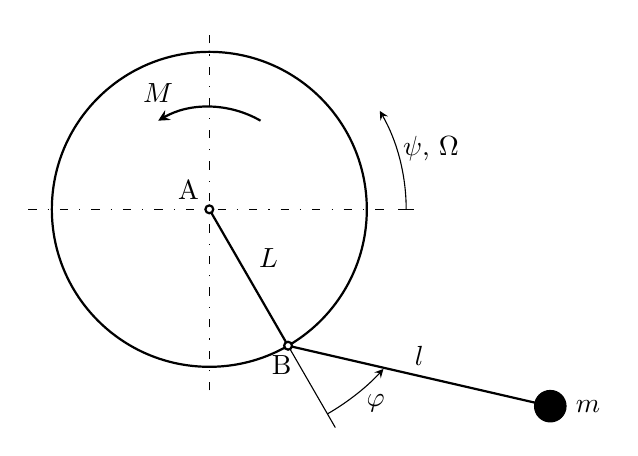
\begin{tikzpicture}[>=stealth]
\draw [loosely dashdotted] (-2.3,0) -- (2.3,0);
\draw [loosely dashdotted](0,-2.3) -- (0,2.3);
\draw [thick] (0,0) circle (2cm);


\draw [thick] (0mm,0mm) -- node[anchor=south west]{$L$} (-60:2);
%\draw (0,0) -- (-60:3);
%\draw [->] (-60:2.8cm) arc (-45:2.8cm:2.8cm);

\draw [->, thick] (60:1.3cm) arc (60:120:1.3cm) node[above=0.1cm]{$M$};

% Bemaßung Omega
\draw [->] (0:2.5cm) arc (0:30:2.5cm) node[right=0.65cm,below=0.2cm]{$\psi$, $\Omega$};
\draw  (2.4,0) -- (2.6,0);

% Bemaßung l und m
\draw  [thick] (-60:2) -- node[anchor=south]{$l$} (-30:5);
\filldraw (-30:5) circle (.2cm) node[right=0.2cm]{$m$};

% Bemaßung Winkel
\draw (-60:2) --  (-60:3.2);
\draw [->] (-60:3cm) arc (-60:-42.5:3cm) node[left=0.1cm, below=0.2cm]{$\varphi$};


% Einfügen der Punkte A und B
\filldraw[fill=white, draw=black, thick] (0,0) circle (0.05cm) node[anchor=south east]{A};
\filldraw[fill=white, draw=black, thick] (-60:2) circle (0.05cm) node[left=0.08cm,below]{B};
\end{tikzpicture}

%	\includegraphics{Grafiken/GEinleitung/Punktmasse.pdf}
	\caption{Prinzipskizze eines einfachen Fliehkraftpendels}
	\label{fig:Einleitung:PendelMitPunktmasse}
\end{figure}
%
%
Wie exemplarisch in \figref{fig:Einleitung:PendelMitPunktmasse} dargestellt ist, bewegt  sich dabei ein solches
Pendel (Masse $m$) auf einer Kreisbahn um einen festen Aufhängepunkt am Rotor \cite{Denman:Tautochronic}.
 \figref{fig:Einleitung:PendelMitPunktmasse} zeigt eine um den Punkt A
 mit Drehzahl $\Omega$ rotierende Welle (Rotor) im Querschnitt.
Mit $\psi$ wird der Verdrehwinkel des Rotors bezeichnet, welcher sich bei konstanter
Rotordrehzahl $\Omega$ zu $\psi = \Omega t$ ergibt.
Im Abstand $L$ vom Mittelpunkt A ist im Aufhängepunkt B die Punktmasse $m$ über einen
idealisiert masselosen Stab der Länge $l$  befestigt.
Die Auslenkung von $m$ relativ zur rotierenden Welle wird mit $\varphi$ bezeichnet.
%
%
%
Durch linearisierte Behandlung des als Punktmasse idealisierten Fliehkraftpendels
nach \figref{fig:Einleitung:PendelMitPunktmasse} resultiert als
Differentialgleichung für kleine Winkel $\varphi$
\begin{equation}
	ml\ddot{\varphi} + m L \Omega^2 \varphi = 0.
\label{eq:Einleitung:DGLLinearisiertesSystem}
\end{equation}
%
%
Die Eigenkreisfrequenz des Fliehkraftpendels ist 
\begin{equation}
	\omega_{F} = \Omega \sqrt{\frac{L}{l}} = k \Omega,
\label{eq:Einleitung:EigenfrequenzFliehkraftpendel}
\end{equation}
welche direkt proportional zur Wellendrehzahl $\Omega$ ist und vom geometrischen Faktor $k=\sqrt{\frac{L}{l}}$,
welcher hier als \new{lineares Tuning}, \new{lineare Tuningordnung} oder \new{lineare Abstimmungsordnung}  
bezeichnet wird, abhängt \cite{Schick:1939:WirkungFliehkraftpendel}.
Das Fliehkraftpendel tilgt die durch Erregung der
Ordnung $k_E$ hervorgerufenen Drehschwingungen, wenn
seine Eigenkreisfrequenz $\omega_{F}$ gleich der Anregungsfrequenz $k_E \Omega$ 
ist \cite{Markert:2010:Fahrzeugschwingung, Schick:1939:WirkungFliehkraftpendel}.
Aus der linearen Theorie resultiert  als Abstimmungsbedingung somit die Relation
%
% 
%
\begin{equation}
	k = k_E,
\label{eq:Einleitung:LineareAbstimmungFliehkraftpendel}
\end{equation}
welche zur Erzielung günstiger Tilgerwirkung einzuhalten ist 
\cite{Schick:1939:WirkungFliehkraftpendel,  Slibar-Desoyer:1954:ZurErzielungOptimaler}.
Für die Wahl $k=k_E$ oszilliert die Pendelmasse in solch einer Art und Weise, 
dass die durch die Masse aufgrund der Fliehkraft erzeugte Momentenwirkung auf die Welle
dem anregenden Moment der Ordnung $k_E$ genau entgegenwirkt
\cite{Desoyer-Slibar:1953:BerechnungVonPendelTilgern,  Paslay:Slibar:1956:OptAusSalomonTilger, 
Schick:1939:WirkungFliehkraftpendel, Slibar-Desoyer:1954:ZurErzielungOptimaler}.
Die Wirkungsweise eines so ausgelegten Fliehkraftpendels ähnelt der eines abgestimmten, translatorischen
Schwingungstilgers  \cite{Vidmar:Feeney:2012:CoulombFriction}. 
Ein besonderer Vorteil eines solchen Fliehkraftpendels ist 
die Unabhängigkeit von der Rotordrehzahl $\Omega$ und somit von der Anregungsfrequenz
bei fester Anregungsordnung $k_E$, welche für einen Verbrennungsmotor in Abhängigkeit der Zylinderzahl konstant ist 
\cite{Schick:1939:WirkungFliehkraftpendel}. 
Damit ist das Pendel in beliebigen Betriebszuständen $\Omega \neq \const$ wirksam und
nicht nur bei einer bestimmten, konstanten Solldrehzahl  $\Omega$
bzw. konstanten Anregungsfrequenz $k_E \Omega$ \cite{Schick:1939:WirkungFliehkraftpendel}. 
%bzw. dem Prinzip zweier über eine Drehfeder mit Drehfedersteifigkeit $k_D$ gekoppelten Massenträgheiten $J_1$ und $J_2$.
%
%
%
Die Wirksamkeit solcher Absorber, bei denen sich die Pendelmasse auf einem Kreispfad bewegt (Kreisbahnpendel),
beschränkt sich allerdings auf den Bereich kleiner Pendelausschläge 
(kleine Winkel $\varphi$ in \figref{fig:Einleitung:PendelMitPunktmasse}).
Nichtlineare Effekte führen jedoch dazu, dass die Absorberfrequenz für große Absorberamplituden von
dieser Amplitude (Größe des Ausschlags von $\varphi$) abhängt \cite{LeeShaw:OnTheCounteraction}, was zur Folge
hat, dass die Wirkungsweise solch einfacher Absorber eingeschränkt ist \cite{ALSUWAIYAN:2002:PerformanceAnd}.
In der praktischen Umsetzung werden Kreisbahnpendel als Zweifadenpendel bzw. Pendel 
mit Doppelaufhängung (Doppelfadenpendel) realisiert \cite{Markert:2010:Fahrzeugschwingung}.


Die Periode eines einfachen Kreisbahnpendels ist bei niedrigen Pendelamplituden unabhängig von der Amplitude 
und wenn das Pendel richtig abgestimmt ist, also die richtige Eigenfrequenz besitzt, 
stellt diese Frequenz auch für größere Absorberamplituden (welche durch
größere Amplituden des anregenden Moments entstehen) die richtige Abstimmung dar.
Dies ist für solche Kreisbahnpendel gültig, bis nichtlineare Effekte, welche zur Änderung der Eigenfrequenz des Pendels führen,
signifikant werden \cite{Denman:Tautochronic, Haddow:2003:ExperimentalInv}.
Bei entsprechenden Werten der Anregungsamplitude vergrößert sich die Absorberperiode
des Kreisbahnpendels auf entsprechend große Werte, dass die lineare Theorie das Verhalten nicht mehr hinreichend
genau beschreibt, was zu einer erhöhten Drehmomentbelastung der Kurbelwelle führt
und bis hin zur Zerstörung führen kann \cite{Denman:Tautochronic}.
Dieser Effekt kann durch bewusstes \new{Mistuning}, 
d.\,h. der beabsichtigten Wahl von  $k \neq k_E$, abgemildert werden  \cite{ALSUWAIYAN:2002:PerformanceAnd}.
Um aber dem eben beschriebenen Verhalten möglichst vollständig vorzubeugen, werden Fliehkraftpendel so 
ausgelegt, dass ihre Periode unabhängig von der Amplitude des anregenden Moments und somit
unabhängig von der Absorberamplitude konstant bleibt \cite{Denman:Tautochronic}.
Durch die Wahl anderer Absorberpfade als eine Kreisbahn kann dies  auch für große 
Amplituden erreicht werden \cite{ALSUWAIYAN:2002:PerformanceAnd}. 
Dazu ist die bislang beschriebene kreisförmige Bahn für die Absorbermasse nicht mehr geeignet  \cite{Denman:Tautochronic}.

Wird die Pendelmasse durch vorgegebene Konturen auf Zykloiden oder Epizykloiden geführt,
können die eben beschriebenen Probleme bei Kreisbahnpendeln vermieden werden 
\cite{Denman:Tautochronic, Lee:TorsionalVibRed}. 
Die praktische Realisierung solcher Pfade ist in 
\cite{Denman:Tautochronic, Mayet:Experimental} dargestellt.
Durch Wahl einer besonderen Epizykloide, der Tautochrone, kann erreicht werden, 
dass die Absorberfrequenz für konstante Rotordrehzahl unabhängig von der Absorberamplitude 
bleibt \cite{Denman:Tautochronic}.
Die Eigenschaften eines tautochronen Absorber wurden eingehend in \cite{Denman:Tautochronic}
untersucht und bieten bedeutende Verbesserungen gegenüber Absorbern, welche sich
auf Kreisbahnen bewegen \cite{Denman:Tautochronic, LeeShaw:OnTheCounteraction}.
In \cite{Denman:Tautochronic} wurden die Absorber allerdings weiterhin als einfache
Punktmassen betrachtet.



Am Lehrstuhl für Angewandte Mechanik an der Technischen Universität München werden
Fliehkraftpendel zur passiven Schwingungsreduktion im Automobilbereich entwickelt.
Vor Kurzem wurden dabei gewonnene Forschungsergebnisse in einem Paper mit Titel
"`Tautochronic Centrifugal Pendulum Vibration Absorbers -- General Design and Analysis"' 
\cite{Mayet:Tautochronic} veröffentlicht. 
Dabei werden die Pendelmassen im Gegensatz zum in \cite{Denman:Tautochronic}
dargestellten tautochronen Entwurf von Fliehkraftpendeln nicht mehr als einfache 
Punktmassen betrachtet. 
Deshalb kann die Absorberdynamik nicht mehr durch die reine Bewegung des Pendelschwerpunkts
beschrieben werden, weshalb die in \cite{Denman:Tautochronic} hergeleiteten geometrischen
Beziehungen nicht mehr verwendet werden können \cite{Mayet:Tautochronic}.
Bei der in \cite{Mayet:Tautochronic} dargestellten Formulierung wird eine Rotation der
Pendel zugelassen und die Wirkung
der Massenträgheiten der Pendel mit in den tautochronen Entwurfsprozess aufgenommen.
Des Weiteren wird ein allgemeiner Ansatz für den tautochronen Absorberentwurf 
vorgeschlagen. 
Diese entwickelte \new{Guideline} erlaubt den einheitlichen Umgang mit einer Vielzahl
von verschiedenen Realisierungen von Fliehkraftpendeln und erweitert 
die bislang verwendeten Entwurfsverfahren \cite{Mayet:Tautochronic}.









%Bis ungefähr 1980 wurden diese einfachen, kreisförmigen Pfade zur Abstimmung der Fliehkraftpendel verwendet \cite{Mayet:Tautochronic}.























\section{Ziel der Arbeit}
%
% Optimales Tuning
In dem in  \cite{Mayet:Tautochronic} vorgeschlagenen Entwurfsformalismus ist keine
Dämpfung berücksichtigt. 
Bei der erweiterten Untersuchung eines auf Grundlage dieser Guideline entworfenen, tautochronen 
Fliehkraftpendels im weiteren Verlauf des Papers wird zusätzlich linear viskose Dämpfung
angesetzt, welche die Systemdynamik beeinflusst.
Die Wirkung des Fliehkraftpendels wird dabei auf Basis von Averaging-Gleichungen
untersucht, welche eine Approximation der stationären Systemantwort  darstellen.
Die Schwingungsreduktionswirkung des entworfenen Absorbers
mit linearem Tuning $k=k_E$ ist durch den Einfluss von viskoser Dämpfung 
bei der Anregungsordnung $k_E$ nicht optimal.
Das Fliehkraftpendel zeigt nicht bei der Anregungsordnung $k_E$ beste Wirkung,
sondern der Punkt bester Absorberwirkung verschiebt sich zu einer 
anderen Anregungsordnung $k_{E,shift}$. 
Je größer die  Dämpfung ist, desto ausgeprägter ist dieser Effekt.
Durch die freie Wahl des Absorbertunings $k$ wird eine Veränderung der Geometrie und somit
eine Veränderung der Dynamik bei weiterhin tautochronem Verhalten erreicht und es kann
dem ungewünschten Einfluss der viskosen Dämpfung entgegengewirkt werden. 
Im Rahmen dieser Arbeit soll das optimale Tuning $k$ eines Fliehkraftpendels
in Abhängigkeit linear viskoser Dämpfung allgemein bestimmt werden.
Besonders im Fokus steht dabei die Herleitung einer  analytischen Bedingung,
mit welcher das optimale Tuning $k$ bestimmt und somit
direkt im Entwurfsprozess berücksichtigt werden kann.

% Rotationsgradient
Durch die in \cite{Mayet:Tautochronic} dargestellte Formulierung kann der
Einfluss von  Rotation eines
Fliehkraftpendels und die Wirkung
der Massenträgheit des Pendels mit in den tautochronen Entwurfsprozess aufgenommen werden.
Die Auslegung eines solchen Rotationspendels wird in \cite{Mayet:Tautochronic} anhand
eines Beispiels veranschaulicht.
Dabei bleibt bei der Wahl des Rotationsgradienten, mit welchem die Absorberwirkung maßgeblich
beeinflusst werden kann, ein Term frei. Dieser Term ist vom Anwender zum Einstellen 
einer gewünschten Pendelwirkung zu wählen, wobei eine beliebige Wahl das tautochrone Verhalten
nicht beeinflusst, jedoch die resultierende Absorberwirkung verändert werden kann.
Dieser Term wird in \cite{Mayet:Tautochronic}  als konstant vorgeschlagen.
Eines der Hauptziele dieser Arbeit ist zu untersuchen, wie ein durch bestimmte Wahl des freien
Terms verallgemeinerter Rotationsgradient das Systemverhalten beeinflusst.
Insbesondere sollen dabei Aussagen zur Optimierung der Pendelwirkung durch
spezielle Wahl des Rotationsgradienten getroffen werden. 

% Nichtlineares Mistuning
Des Weiteren ist bekannt, dass die Absorberwirkung durch nichtlineares Mistuning 
erheblich beeinflusst werden kann \cite{Mayet:CPVAMitMistuning}. 
In \cite{Mayet:CPVAMitMistuning} wird ein Ansatz für das nichtlineare Mistuning vorgeschlagen,
welcher direkt in die Guideline aus \cite{Mayet:Tautochronic} aufgenommen werden kann,
jedoch noch nicht im Detail untersucht wurde.
Im Rahmen dieser Arbeit soll der Einfluss von nichtlinearem Mistuning nach dem 
in \cite{Mayet:CPVAMitMistuning} vorgeschlagenen Ansatz auf das Systemverhalten analysiert werden.
Dabei stehen zunächst qualitative Aussagen im Vordergrund. Allerdings sollen
aus den dadurch gewonnenen Erkenntnissen Vorschläge zur gezielten Beeinflussung
des Verhaltens der Fliehkraftpendel unter Berücksichtigung von nichtlinearem Mistuning
abgeleitet werden.




% Lösen der Averaging-Gleichung mit Bogenlängenverfahren
Um die bislang beschriebenen Hauptziele erreichen zu können, müssen die
in  \cite{Mayet:Tautochronic} hergeleiteten, nichtlinearen Averaging-Gleichungen gelöst werden.
Bei den numerischen Untersuchungen in \cite{Mayet:Tautochronic} wurden
die Averaging-Gleichungen, welche eine Approximation der stationären Systemantwort 
darstellen, für Spezialfälle gelöst.
Um dies aber auch für allgemeinere Fälle zu ermöglichen, muss die Lösung
der Averaging-Gleichungen mit einer Methode erfolgen, welche eine systematische Berechnung 
der stationären Systemantwort für alle Arten von Fliehkraftpendeln erlaubt.
Ein hierfür geeignetes Verfahren ist das Bogenlängenverfahren, welches im
Rahmen dieser Arbeit auf die Averaging-Gleichungen angewendet werden soll.
%Die damit erzielten Ergebnisse ermöglichen es, Aussagen über das stationäre
%Systemverhalten zu treffen  und können für den systematischen Auslegungsprozess
%von Fliehkraftpendeln genutzt werden.

% Vollständige Simulation der Bewegungsgleichungen
Um die Aussagekraft der auf Basis der Averaging-Gleichungen hergeleiteten Zusammenhänge
beurteilen zu können, sollen diese Ergebnisse durch die  Simulation der 
vollständigen, nicht vereinfachten, nichtlinearen Bewegungsgleichungen des
dynamischen Fliehkraftpendelsystems verifiziert werden. 
Dazu müssen die vollständigen Bewegungsgleichungen auf eine Art und Weise implementiert werden,
dass die erhaltenen Simulationsergebnisse direkt mit den 
Resultaten aus den Averaging-Gleichungen verglichen werden können.


% Zusammenfassender Satz
Im Rahmen dieser Arbeit soll auf Basis der Averaging-Gleichungen, deren
Aussagekraft durch anschließende Simulation der vollständigen, nichtlinearen Bewegungsgleichungen
beurteilt wird, das optimale lineare Tuning $k$ bestimmt,
der Einfluss eines verallgemeinerten Rotationsgradienten und die Berücksichtigung von 
nichtlinearem Mistuning auf das Systemverhalten untersucht werden. 









\section{Gliederung der Arbeit}


% Theorieteil, Kapitel 2
In \chref{ch:StandDerForschung} werden die theoretischen Grundlagen auf Basis der kürzlich
veröffentlichten Forschungsergebnisse \cite{Mayet:Tautochronic}, 
worauf in  dieser Arbeit aufgebaut wird, dargestellt.
Hierzu wird in \secref{sec:TautochronerEntwurfAllgemein} die entwickelte Formulierung
für den tautochronen Absorberentwurf dargelegt. 
Die Veranschaulichung der Sachverhalte, welche für diese Arbeit
grundlegend sind und auf welchen im weiteren Verlauf aufgebaut wird bzw.
worauf sich an späterer Stelle wieder bezogen wird, steht dabei im Vordergrund.
Es wird ein Einblick auf den grundlegenden Hintergrund dieser Arbeit gegeben.
Weiterführende Herleitungen und detaillierte Informationen können \cite{Mayet:Tautochronic} entnommen werde.
Anschließend wird in \secref{sec:TheorieMistuning} der in \cite{Mayet:CPVAMitMistuning} vorgeschlagene
Mistuning-Ansatz eingeführt. Dabei werden die Auswirkungen durch Berücksichtigung von nichtlinearem
Mistuning auf den in \cite{Mayet:Tautochronic} gegebenen Formalismus aufgezeigt.


% Vollständige Simulation
Um die Aussagekraft der auf Basis der Averaging-Gleichungen hergeleiteten Zusammenhänge
beurteilen zu können, wird  in \chref{cha:VollstaendigSimulation}
auf die Simulation der  vollständigen, nichtlinearen Bewegungsgleichungen 
von Fliehkraftpendelsystemen eingegangen.
Hierfür wird in \secref{sec:BewegungsgleichungenInMatlab} der strukturelle Aufbau der Bewegungsgleichungen 
nach dem Lagrange-Formalismus hergeleitet und
alle benötigten Terme explizit ermittelt, um ein vollständig bestimmtes Differentialgleichungssystem 
zur Implementierung zu erhalten.
Anschließend  wird auf Details und Besonderheiten bei der Implementierung 
in \textsc{Matlab} eingegangen (\secref{sec:ImplementierungInMatlab}).
Im Vordergrund steht dabei, dass die aus der Simulation des nichtlinearen Differentialgleichungssystems 
resultierenden Größen direkt mit den aus den Averaging-Gleichungen 
bestimmten Ergebnissen verglichen werden können. 
Dieses Kapitel wird dem darauffolgenden \chref{cha:LoesenAverGl} zur Lösung der Averaging-Gleichungen vorangestellt,
da zur vollständigen Bestimmung des Differentialgleichungssystems Ausdrücke hergeleitet werden,
welche im Anschluss bei der Lösung der Averaging-Gleichungen wiederverwendet werden können.


% Bogenlängenverfahren
Zur systematischen Lösung der Averaging-Gleichungen wird in \chref{cha:LoesenAverGl} das
Bogenlängenverfahren verwendet.
Zunächst wird  in  \secref{sec:Bogenlangenverfahren} der Grundgedanke des Verfahrens dargelegt 
und es werden grundlegende Vorteile des Verfahrens aufgezeigt. 
Bei der Herleitung wird die ursprüngliche, strukturmechanisch geprägte Terminologie verwendet und anschließend
auf die in den Averaging-Gleichungen auftretenden Größen übertragen.
Das Prinzip zur Lösung  der Averaging-Gleichungen wird  am 
Beispiel eines Absorbers demonstriert (\secref{sec:Bogenlaenge:UebertrafAufAveragingGleichungen}).
In \secref{sec:Bogenlange:Implementierung} wird auf  die praktische Umsetzung des Bogenlängenverfahrens eingegangen
und die Implementierung des Verfahrens in \textsc{Matlab} veranschaulicht.


% Optimales Tuning
Auf die allgemeine  Bestimmung des optimalen Tunings $k$ eines Fliehkraftpendels
in Abhängigkeit linear viskoser Dämpfung wird in \chref{cha:Optimierung} eingegangen.
Dabei wird zunächst in \secref{sec:Opt:SuboptDurchDaempfung}  aufgezeigt, wie die
Berücksichtigung von Dämpfung das Systemverhalten beeinflusst, wodurch
die Absorberperformance bei der Anregungsordnung $k_E$ nicht optimal ist.
Durch entsprechende Wahl des Absorbertunings kann die
bestmögliche Absorberwirkung dennoch bei der gewünschten Anregungsordnung erreicht werden.
Wie das Tuning explizit zu wählen ist, wird in  \secref{sec:Opt:BedingungFuerMinimum} veranschaulicht.
Anschließend wird in  \secref{sec:Opt:Bsp}
die Anwendung der hergeleiteten Zusammenhänge an einem Beispiel demonstriert.


% Untersuchung Rotationsgradient
In \chref{cha:EinflussRotGrad} wird der Einfluss eines verallgemeinerten
Rotationsgradienten auf das Systemverhalten untersucht.
Zunächst wird in \secref{sec:RotGrad:Ansatz} der verallgemeinerte Ansatz vorgestellt
und es werden die Auswirkungen auf andere funktionale Zusammenhänge im Entwurfsprozess dargelegt.
In \secref{sec:RotGrad:EinflussEinzelneTerme} wird der Einfluss dieses Ansatzes 
auf das Systemverhalten untersucht und anschließend wird in \secref{sec:UntersVariabRotGrad:GezielteMinimierung}
aufgezeigt, wie das Verhalten durch spezielle Wahl des Rotationsgradienten gezielt beeinflusst werden kann. 
Die durch die Averaging-Gleichungen prognostizierten Verbesserungen der Absorberperfor\-mance werden
in \secref{sec:RotGrad:VergleichSimulation} mit der vollständigen Simulation verglichen. 
%Da es hier zu deutlichen Abweichung kommt, scheinen die Averaging-Gleichung das Systemverhalten
%unter den dort getroffenen Annahmen nicht sonderlich gut zu approximieren.
In \secref{sec:RotGrad:BeruecksichtungTermeHoehererOrdnung} wird durch die Verwendung von 
Ansätzen höherer Ordnung die Approximation durch die Averaging-Gleichungen verbessert und aus den
daraus resultierenden Ergebnissen eine Aussage über das
optimale Verhalten eines Rotationspendels  getroffen.


% Untersuchung Mistuning
Die in \chref{cha:UntersuchungenMistuning} durchgeführten Untersuchungen zum Einfluss von nichtlinearem
Mistuning auf Basis der Averaging-Gleichungen  werden anhand eines Absorbers unter Verwendung
der Ergebnisse aus \chref{cha:EinflussRotGrad} demonstriert.
Dabei wird in \secref{sec:UntersMist:AnsatzMistuning} der verwendete Ansatz für das
nichtlineare Mistuning $u(s)$ vorgestellt und in \secref{sec:UntersMist:EinflussAufAverGl} der Einfluss dieses Ansatzes 
auf das Systemverhalten untersucht. Es wird aufgezeigt, wie das stationäre Verhalten des 
zugrunde liegenden Systems gezielt beeinflusst werden kann.
Die auf Basis der Averaging-Gleichungen prognostizierte Verbesserung der Fliehkraftpendelwirkung wird
in \secref{sec:Mistuning:AblgeichVollStSimul} mit der vollständigen Simulation verglichen.
%, wobei äußerste gute Übereinstimmung resultiert.
%
Daraus werden anschließend Folgerungen für den Absorberentwurf unter Berücksichtigung von
nichtlinearem Mistuning getroffen und
abschließend in \secref{sec:UntersMist:Einsatzmoeglichkeiten} exemplarisch aufgezeigt,
wie das Systemverhalten gezielt durch den Einsatz von nichtlinearem Mistuning beeinflusst werden kann.



% Schluss
\chref{cha:Schluss} fasst die wichtigsten Aspekte dieser Arbeit zusammen und gewährt einen Ausblick
auf Anwendungen und mögliche Erweiterungen.

















%\section{Tests}



%Textwidth: \the\textwidth 


%action-angle-Variablen: \cite{markus:1974:generic}

%und hier noch der Hagedorn \cite{Hagedorn:NichtlinSchwingungen1978}






%%%%%%%%%%%%%%%%%%%%%%%%%%%%%%%%%%%%%%%%%%%%%%%%%%%%%%%%%%%%%%%%%%%%%%%%%
% ZUNÄCHST ANGEDACHTE ERLÄUTERUNGEN
%%%%%%%%%%%%%%%%%%%%%%%%%%%%%%%%%%%%%%%%%%%%%%%%%%%%%%%%%%%%%%%%%%%%%%%%%



%
%Zwei Massen verbunden mit Feder (einfachst möglicher Fall, um Prinzip zu skizzieren):
%
%Periodische Anregung: 
%\begin{equation}
	%F(t) = F_0 \sin \left( \Omega t \right)
%\label{eq:PeriodischAnregendeKraft}
%\end{equation}
%
%%
%%
%%
%Bewegungsgleichungen:
%% 
%\begin{subequations}
	%\begin{align}
		%m_1 \ddot{x}_1 & = -k_{F} \left( x_1 - x_2 \right) + F_0 \sin \left( \Omega t \right) \\
		%m_2 \ddot{x}_2 & = k_{F} \left( x_1 - x_2 \right)
	%\end{align}
	%\label{eq:BewegungsleichungenTranslatorischerSchwingungstilger}	
%\end{subequations}
%
%%\begin{figure}[ht]
	%%\centering
	%%\def\svgwidth{0.3\textwidth}
	%%\import{./Grafiken/Zeichnung2/}{Versuch3.pdf_tex}
	%%\caption{Prinzipskizze eines Schwingungstilgers (translatorisch)}
%%\end{figure}
%
%
%Für stationäre Lösungen der fremderregten Schwingung resultiert mit
%\begin{equation}
		%x_1 = \hat{x}_{1} \sin \left( \Omega t \right), \qquad x_2 = \hat{x}_{2} \sin \left( \Omega t \right) 
	%\label{eq:BewegungsleichungenTranslatorischerSchwingungstilgerLoesungsansatz}	
%\end{equation}
%
%für die Amplitude $\hat{x}_{1}$ (hier noch ein Zitat hin)
%\begin{equation}
		%\hat{x}_{1} = \frac{F_0  \left(k_{F} - m_2 \Omega^2\right) }{m_1 m_2 \Omega^2 \left[ \Omega^2 - k_{F} \left(\frac{1}{m_1} + \frac{1}{m_2} \right) \right]} 
	%\label{eq:AmplitudeTranslatorischerSchwingungstilger}	
%\end{equation}
%
%
%Der prinzipielle Verlauf von $\hat{x}_{1}$ über $\Omega$ ist in (xxx) dargestellt. 
%
%%\begin{figure}[ht]
	%%\centering
	%%\def\svgwidth{\textwidth}
	%%\import{./Grafiken/Zeichnung2/}{Test1.pdf_tex}
	%%\caption{Amplitudenverlauf über $\Omega$}
%%\end{figure}
%
%
%
%
%
%
%
%%\begin{figure}[ht]
	%%\centering
	%%\def\svgwidth{0.5\textwidth}
	%%\import{./Grafiken/Zeichnung2/}{Drehfeder1.pdf_tex}
	%%\caption{Prinzipskizze eines Schwingungstilgers (translatorisch)}
%%\end{figure}
%
%
%
%%
%%
%%%%%%%%%%%%%%%%%%%%%%%%%%%%%%%%%%%%%%%%%%%%%
%% jetzt Torsionsschwinungen
%%%%%%%%%%%%%%%%%%%%%%%%%%%%%%%%%%%%%%%%%%%%%
%%
%%
%\newcommand{\WinkelA}{\beta}
%analog kann dies für Torsionsschwingungen hergeleitet werden \cite[Anhang A]{Denman:Tautochronic}, wobei Massen durch Massenträgheitsmomente, translatorische Freiheitsgrad durch rotatorische Freiheitsgrade und die Federsteifigkeit durch eine Drehfedersteifigkeit ersetzt werden, womit sich die folgenden Bewegungsgleichungen ergeben
%%
%%
%% Bewegungsgleichungen
%%
%\begin{subequations}
	%\begin{align}
		%\Theta_1 \ddot{\WinkelA}_1 & = -k_{D} \left( \WinkelA_1 - \WinkelA_2 \right) + M_0 \sin \left( \Omega t \right) \\
		%\Theta_2 \ddot{\WinkelA}_2 & = k_{D} \left( \WinkelA_1 - \WinkelA_2 \right)
	%\end{align}
	%\label{eq:BewegungsleichungenLinearerTorsionsschwingungsAbsorber}%	
%\end{subequations}
%%
%%
%und für die stationäre Lösung mit Ansatz  $\WinkelA_1 = \hat{\WinkelA}_{1} \sin \left( \Omega t \right)$, $\WinkelA_2 = \hat{\WinkelA}_{2} \sin \left( \Omega t \right)$ sich der Amplitudenverlauf
%%
%%
%%
%\begin{equation}
		%\hat{\WinkelA}_{1} = \frac{M_0  \left(k_{D} - \Theta_2 \Omega^2\right) }{\Theta_1\Theta_2 \Omega^2 \left[ \Omega^2 - k_{D} \left(\frac{1}{\Theta_1} + \frac{1}{\Theta_2} \right) \right]} 
	%\label{eq:AmplitudeRotatorischerSchwingungstilger}	
%\end{equation}
%und somit die Resonanzkurve analog ergibt. Anhand von Gleichung 	\eqref{eq:AmplitudeRotatorischerSchwingungstilger}	 ist klar ersichtlich, dass die Amplitude für
%%
%%
%% Verschwinden der Amplitude
%%
%\begin{equation}
		%k_{D} = \Theta_2 \Omega^2
	%\label{eq:AmplitudeRotatorischerSchwingungstilgerBedinungungfuerVerschwinden}	
%\end{equation}
%verschwindet




\chapter{Stand der Forschung} \label{ch:StandDerForschung}

Es soll ein Einblick auf den grundlegenden Hintergrund dieser Arbeit gegeben werden.
Deshalb wird in \secref{sec:TautochronerEntwurfAllgemein} die in \cite{Mayet:Tautochronic} entwickelte Formulierung
für den tautochronen Absorberentwurf dargelegt. 
Die Veranschaulichung der Sachverhalte, welche für diese Arbeit
grundlegend sind, steht dabei im Vordergrund.
Anschließend wird in \secref{sec:TheorieMistuning} der in \cite{Mayet:CPVAMitMistuning} vorgeschlagene
Mistuning-Ansatz eingeführt. Dabei werden die Auswirkungen des nichtlinearen
Mistuning-Ansatzes auf den zuvor in \secref{sec:TautochronerEntwurfAllgemein} skizzierten Formalismus aufgezeigt.


\section{Tautochroner Entwurf von Fliehkraftpendeln } 

\label{sec:TautochronerEntwurfAllgemein}


Die in diesem Abschnitt dargelegten Zusammenhänge stammen aus dem 
kürzlich veröffentlichten Paper \cite{Mayet:Tautochronic}.
Es werden die Sachverhalte veranschaulicht, welche für diese Arbeit
grundlegend sind und auf welchen im weiteren Verlauf aufgebaut wird bzw.
worauf sich an späterer Stelle wieder bezogen wird.
Dabei wird ein Einblick auf den grundlegenden Hintergrund dieser Arbeit gegeben,
ohne jedoch sämtliche Herleitungen und detaillierte Informationen wiederzugeben.
Für eine ausführliche und vollständige Darstellung sei an dieser Stelle
auf  \cite{Mayet:Tautochronic} verwiesen.


% Referenzen auf Gleichungen einfügen









\subsection[Systembeschreibung]{Systembeschreibung\footnote{Kapitel 3 in \cite{Mayet:Tautochronic}}}


\label{subsec:Systembeschreibung}



%%%%%%%%%%%%%%%%%%%%%%%%%%%%%%%%%%%%%%%%%%%%%%%%%%%%%%%%%%%%%%%%%%%%%%%%%%%%%%%%%%
% Ursprüngliche, viel ausführlichere Version
%%%%%%%%%%%%%%%%%%%%%%%%%%%%%%%%%%%%%%%%%%%%%%%%%%%%%%%%%%%%%%%%%%%%%%%%%%%%%%%%%%
%\subsubsection{Kinetische Energie}

Das in	\figref{fig:Theorie:BildCPVA} dargestellte Fliehkraftpendel
wird als Basis für die mathematische Beschreibung des mechanischen Systems
verwendet \cite{Mayet:Tautochronic}. Details zu diesem Fliehkraftpendeltyp sind
in \cite{mayet2012euromech} und Informationen zu damit durchgeführten, experimentellen Untersuchungen 
in \cite{Mayet:Experimental} zu finden.
%
%
\begin{figure}[ht]%
	\centering
			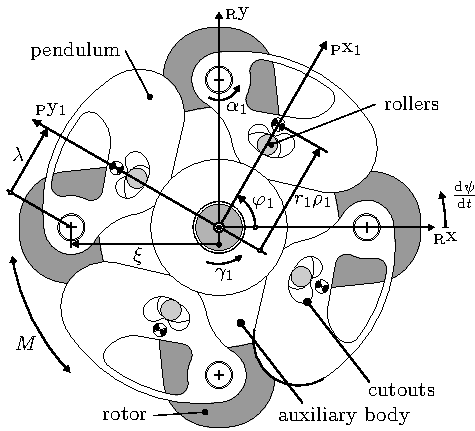
\includegraphics{PIC_120209_schematic_scpa_make}
			\caption[Schematische Darstellung eines Fliehkraftpendels]{Schematische Darstellung eines Fliehkraftpendels \cite{mayet2012euromech}}
	\label{fig:Theorie:BildCPVA}
\end{figure}
%
%
%
Der Rotor mit Freiheitsgrad $\psi(t)$ besitzt das Massenträgheitsmoment $\Theta_{Rotor}$.
Das dargestellte Absorbersystem besteht aus $n_p=4$ Pendeln, aus einem Hilfskörper ($n_a=1$)
und zugehörigen Wälzkörpern. 
Durch die kinematische Kopplung der vier Pendel über Hilfs- und Wälzkörper besitzt
das Fliehkraftpendelsystem nur einen Freiheitsgrad, welcher durch die generalisierte Koordinate $s(t)$
beschrieben wird. 
%
Jedes Pendel (Masse $m_i$, Massenträgheitsmoment $\Theta_{S,i}$ bezüglich seines Schwerpunkts und
Abstand $r_i \rho_i$ vom Drehpunkt des Rotors) kann Rotationen $\alpha_i(s)$ relativ
zum rotorfesten Koordinatensystem  $(\rs{_R}{x},\rs{_R}{y},\rs{_R}{z})$ ausführen. 
Die relative Rotation des Hilfskörpers (Massenträgheitsmoment $\Theta_{A,1}$ bezüglich seines Schwerpunkts)
wird mit $\gamma_1(s)$ bezeichnet und der Schwerpunkt des Hilfskörpers befindet sich in seinem
Drehpunkt. Dieser fällt mit dem Rotordrehpunkt zusammen, weshalb der Hilfskörper nur rotatorische
Bewegungen ausführen kann. Im allgemeinen Fall können beliebig viele Hilfskörper $n_a$ verwendet werden.
%
Der Winkel $\varphi_i (s)$ ist der Winkel zwischen dem rotorfesten Koordinatensystem 
$(\rs{_R}{x},\rs{_R}{y},\rs{_R}{z})$ und dem Koordinatensystem $(\rs{_P}[_i]{x},\rs{_P}[_i]{y},\rs{_P}[_i]{z})$, 
wobei der Schwerpunkt des $i$-ten Pendels auf der $\rs{_P}[_i]{x}$-Achse liegt.
%
Durch die Kontur der Ausfräsungen im Pendel und im Hilfskörper  können 
durch die kinematische Kopplung über die Wälzkörper beliebige,
nichtlineare, kinematische Zusammenhänge zwischen $\alpha_i(s)$ und $\gamma_1(s)$ vorgegeben werden.



Die Zeit $t$ wird in den folgenden Ausführungen mit der Mitteldrehzahl $\Omega$ des Rotors
skaliert und der Einfluss der Dynamik der Wälzkörper vernachlässigt.
Die skalierte Zeit wird mit $\tau = \Omega t$ bezeichnet und für Ableitungen 
nach $\tau$ wird die Abkürzung $ \dot{\left(\bullet\right)} =\frac{\dd}{\dd{\tau}}\left(\bullet\right)$ verwendet.

Die gesamte kinetische Energie $T_{tot}$ des Systems setzt sich aus den kinetischen Energien der einzelnen Körper zusammen
und ergibt sich zu
%
% Gesamte kinetische Energie
%
\begin{equation}
	T_{tot} = T_R + \sum_{i=1}^{n_p} T_{P,i} + \sum_{j=1}^{n_a} T_{A,j},
\label{eq:GesamteKinetischeEnergieTtot}
\end{equation}
%
%
%
wobei $T_R = \frac{1}{2}\Theta_{Rotor} \Omega^2 \dot{\psi}^2$ die kinetische Energie des Rotors, 
$T_{P,i}$ die kinetische Energie des $i$-ten Pendels 
\begin{equation}
	T_{P,i} = \frac{1}{2} m_i r_i^2 \left( \left(\pdiff{\rho_i}{s}\right)^2 \dot{s}^2 + \rho_i^2 \left(\pdiff{\varphi_i}{s}\dot{s}+\dot{\psi}\right)^2 \right) \Omega^2 
						+ \frac{1}{2} \Theta_{S,i} \left( \pdiff{\alpha_i}{s}\dot{s} + \dot{\psi} \right)^2 \Omega^2
\label{eq:KinetischeEnergiePendel}
\end{equation}
und $T_{A,j}$ die kinetische Energie des $j$-ten Hilfskörpers 
\begin{equation}
	T_{A,j} = \frac{1}{2} \Theta_{A,j} \left( \pdiff{\gamma_j}{s}\dot{s} + \dot{\psi} \right)^2 \Omega^2
\label{eq:KinetischeEnergieAuxiliaryBody}
\end{equation}
bezeichnet. $\rho_i (s)$ mit $\rho_i (0) = 1$ stellt den skalierten Abstand des $i$-ten Pendelschwerpunkts 
vom Rotordrehpunkt in Richtung der $\rs{_P}[_i]{x}$-Achse dar.
%
%
%
%
%%%%%%%%%%%%%%%%%%%%%%%%%%%%%%%%%%%%%%%%%%%%%%%%%%%%%%%%%%%%%%%%%%%%%%%%%%%%%%%%%%
%%%%%%%%%%%%%%%%%%%%%%%%%%%%%%%%%%%%%%%%%%%%%%%%%%%%%%%%%%%%%%%%%%%%%%%%%%%%%%%%%%
% Ursprüngliche, viel ausführlichere Version
%%%%%%%%%%%%%%%%%%%%%%%%%%%%%%%%%%%%%%%%%%%%%%%%%%%%%%%%%%%%%%%%%%%%%%%%%%%%%%%%%%
%%%%%%%%%%%%%%%%%%%%%%%%%%%%%%%%%%%%%%%%%%%%%%%%%%%%%%%%%%%%%%%%%%%%%%%%%%%%%%%%%%
%
% Kinetische Energie eines Hilfskörpers
%
%Der Hilfskörper $j$ mit Massenträgheitsmoment $\Theta_{A,j}$ kann nur rein rotatorische Bewegungen ausführen, weshalb sich dessen kinetische Energie zum einen aus dem Anteil der Rotation des rotorfesten Koordinatensystems $(\rs{_R}{x},\rs{_R}{y},\rs{_R}{z})$ und zum anderen aus dem Anteil der Drehung des Hilfskörpers $j$ um den Winkel $\gamma_j$ relativ zum rotorfesten Koordinatensystem zusammensetzt. 
%Die kinetische Energie $T_{A,j}$ des $j$-ten Hilfskörpers lautet
%\begin{equation}
%	T_{A,j} = \frac{1}{2} \Theta_{A,j} \left( \pdiff{\gamma_j}{s}\dot{s} + \dot{\psi} \right)^2 \Omega^2.
%\label{eq:KinetischeEnergieAuxiliaryBody}
%\end{equation}
%
%
% Kinetische Energie eines Pendels
%
%Die kinetische Energie des $i$-ten Pendels setzt sich sowohl aus translatorischen als auch aus rotatorischen Anteilen zusammen und kann unter Verwendung der bisher eingeführten Größen als
%\begin{equation}
%	T_{P,i} = \frac{1}{2} m_i r_i^2 \left( \left(\pdiff{\rho_i}{s}\right)^2 \dot{s}^2 + \rho_i^2 \left(\pdiff{\varphi_i}{s}\dot{s}+\dot{\psi}\right)^2 \right) \Omega^2 + \frac{1}{2} \Theta_{S,i} \left( \pdiff{\alpha_i}{s}\dot{s} + \dot{\psi} \right)^2 \Omega^2
%\label{eq:KinetischeEnergiePendel}
%\end{equation}
%geschrieben werden, wobei $\rho_i (s)$ mit $\rho_i (0) = 1$ den skalierten Abstand in Richtung der $\rs{_P}[_i]{x}$-Achse darstellt. Der Winkel $\varphi_i\left(s\right)$ ist der Winkel zwischen dem rotorfesten Koordinatensystem $(\rs{_R}{x},\rs{_R}{y},\rs{_R}{z})$ und dem Koordinatensystem $(\rs{_P}[_i]{x},\rs{_P}[_i]{y},\rs{_P}[_i]{z})$, wobei der Schwerpunkt des $i$-ten Pendels auf der $\rs{_P}[_i]{x}$-Achse liegt.
%
%
%%%%%%%%%%%%%%%%%%%%%%%%%%%%%%%%%%%%%%%%%%%%%%%%%%%%%%%%%%%%%%%%%%%%%%%%%%%%%%%%%%
%%%%%%%%%%%%%%%%%%%%%%%%%%%%%%%%%%%%%%%%%%%%%%%%%%%%%%%%%%%%%%%%%%%%%%%%%%%%%%%%%%
%
%
%
%
%
% Potential
%
Durch die spezielle Anwendung der Fliehkraftpendel zur Schwingungsreduktion bei Viertaktmotoren, bei welchen 
sich der Zylinderzyklus alle zwei Umdrehungen wiederholt, kann das anregende, externe Moment in Abhängigkeit
des Rotorwinkels $\psi$ geschrieben werden. Die potentielle Energie $V = V(\psi)$ lautet dann
\begin{equation}
		V\left(\psi\right) = - \int^{\psi}_{0} {M\left(\bar{\psi}\right) \dd \bar{\psi}} = M_0 \sin \left(k_E \psi\right) ,
\label{eq:PotentialDesAnregendenMoments}
\end{equation}
wobei das anregende Moment $M\left(\psi\right) = -k_E M_0 \cos \left(k_E \psi\right)$, welches auf den Rotor wirkt, 
als harmonische Anregung der Ordnung $k_E$ mit Amplitude $M_0$ angenommen wird (vgl. \secref{sec:Einl:Motivation}).
%
%
Für die Lagrange-Funktion $L = T_{tot} - V$ des betrachteten Systems resultiert dann
\begin{equation}
\begin{split} 
	L & = T_{tot} - V = T_R  + \sum_{j=1}^{n_a} T_{A,j} - V  + \sum_{i=1}^{n_p} T_{P,i} \\
		& = \frac{1}{2}\Theta_{Rotor} \Omega^2 \dot{\psi}^2 + \sum_{j=1}^{n_a} \left[\frac{1}{2} \Theta_{A,j} \left( \pdiff{\gamma_j}{s}\dot{s} + \dot{\psi} \right)^2 \Omega^2\right] - M_0 \sin \left(k_E \psi\right) \\
		& + \sum_{i=1}^{n_p} \left[\frac{1}{2} m_i r_i^2 \left( \left(\pdiff{\rho_i}{s}\right)^2 \dot{s}^2 + \rho_i^2 \left(\pdiff{\varphi_i}{s}\dot{s}+\dot{\psi}\right)^2 \right) \Omega^2 + \frac{1}{2} \Theta_{S,i} \left( \pdiff{\alpha_i}{s}\dot{s} + \dot{\psi} \right)^2 \Omega^2\right].   \end{split}
	\label{eq:LagrangeFunktionInRealenKoordinaten}
\end{equation}
%
%
%
%
%
%
%
%
%
%
%
%
%
%
%
%
%
%
%
%
%
%
%
%
%
%
%
%
%
%
%
%
%
%
%
%%%%%%%%%%%%%%%%%%%%%%%%%%%%%%%%%%%%%%%%%%%%%%%%%%%%%%%%%%%%%%%%%%%%%%%%%%%%%%%%%%
% Ursprüngliche, viel ausführlichere Version
%%%%%%%%%%%%%%%%%%%%%%%%%%%%%%%%%%%%%%%%%%%%%%%%%%%%%%%%%%%%%%%%%%%%%%%%%%%%%%%%%%
%\subsubsection{Skalierte Lagrange-Funktion}
%
Um  eine dimensionslose Darstellung für die einheitliche Systembetrachtung zu erhalten, wird Gleichung
\eqref{eq:LagrangeFunktionInRealenKoordinaten} mit $1/({\Theta_{Scale}\Omega^2})$ 
durchmultipliziert.
Dies führt nach  \cite{Mayet:Tautochronic} auf die \new{skalierte Lagrange-Funktion} 
$\tilde{L} = (T_{tot} - V)/(\Theta_{Scale}\Omega^2)$, welche als
%
\begin{equation}
\begin{split}  
	\tilde{L} &= \frac{1}{2} \epsilon^{-1} \dot{\psi}^2 + \frac{1}{2} \sum_{i=1}^{n_p} \left( \mu_{m,i}  \left( \left( \pdiff{\rho_i}{s} \right)^2 \dot{s}^2 + \rho_i^2 \left( \pdiff{\varphi_i}{s} \dot{s} 
																																											+ \dot{\psi} \right)^2 \right) + \mu_{r,i} \left( \pdiff{\alpha_i}{s} \dot{s} + \dot{\psi} \right)^2 \right) \\
						&+ \frac{1}{2} \sum_{i=1}^{n_a} \nu_j \left( \pdiff{\gamma_j}{s} \dot{s} + \dot{\psi} \right)^2  - \Gamma \sin\left( k_E \psi \right) \end{split}
\label{eq:SkalierteLagrangeFunktionfuereinAbsorbersystem}
\end{equation}
%
mit den abkürzenden Schreibweisen
%
\begin{equation}
\begin{split} 	\Theta_{Scale}&= \max \left( m_1 r_1^2, m_2 r_2^2, \dots, m_{n_p} r_{n_p}^2 \right),&		\Gamma&= \frac{M_0}{\Theta_{Scale} \Omega^2},& 			\nu_j&= \frac{\Theta_{A,j}}{\Theta_{Scale}},\\ 
								\mu_{m,i}&= \frac{m_i r_i^2}{\Theta_{Scale}},& 																					\mu_{r,i}&= \frac{\Theta_{S,i}}{\Theta_{Scale}},& 	\epsilon&= \frac{\Theta_{Scale}}{\Theta_{Rotor}} \end{split}
\label{eq:SkalierteLagrangeFunktionAbkuerzungen}
\end{equation}
%
geschrieben wird, was zur Vereinheitlichung und Vereinfachung des Entwurfsprozesses
beliebiger Fliehkraftpendeltypen dienen kann \cite{Mayet:Tautochronic}.
%
%
%
%
%
%
% Bedingungen an rho, bzw. s (s_cusp)
%
%\begin{equation}
	%\rho_i(s=0) = 1 
	%\label{eq:SkalierteRadiusVons=0muss1sein}
%\end{equation}
Die skalierten Radien $\rho_i$ sind sinnvollerweise auf das Intervall 
\begin{equation}
	\rho_i(s) \in [0,\:1] 
	\label{eq:SkalierteRadiusImIntevall0bis1}
\end{equation}
beschränkt und bedingt durch den spezifischen Absorberentwurf liegt darüber hinaus für $s \in \MR$  
eine geometrische Begrenzung $s_{cusp}$
\begin{equation}
	\left|s(\tau)\right| \leq s_{cusp} \in \MR^+ \quad \forall \tau \in \MR^+  
	\label{eq:BeschraenkungAnSDurchScusp}
\end{equation}
für die Absorberamplitude vor \cite{Mayet:Tautochronic}.






%%%%%%%%%%%%%%%%%%%%%%%%%%%%%%%%%%%%%%%%%%%%%%%%%%%%%%%%%%%%%%%%%%%%%%%%%%%%%%%%%%
% Ursprüngliche, viel ausführlichere Version
%%%%%%%%%%%%%%%%%%%%%%%%%%%%%%%%%%%%%%%%%%%%%%%%%%%%%%%%%%%%%%%%%%%%%%%%%%%%%%%%%%
% \subsubsection{Bewegungsgleichungen}
%
% Bewegungsgleichungen nach Lagrange
%
%Die Ableitung der vollständigen Bewegungsgleichungen erfolgt im Folgenden mittels Lagrange-Formalismus $\frac{\dd}{\dd \tau} \pdiff{\tilde{L}}{{\dot{q}_i}} - \pdiff{\tilde{L}}{{q_i}} = 0$
%unter der Annahme eines konservativen Systems mit zugehöriger Lagrange-Funktion wie in \eqref{eq:SkalierteLagrangeFunktionfuereinAbsorbersystem} angegeben. Es werden die generalisierten Koordinaten $\vq = [\psi \quad s]^T$ und deren Ableitungen $\vec{\dot{q}} = [\dot{\psi} \quad \dot{s}]^T$ verwendet. Zunächst resultieren für das vorliegende System die Differentialgleichungen 
%
%
%%%%%%%%%%%%%%%%%%%%%%%%%%%%%%%%%%%%%%%%%%%%%%%%%%%%%%%%%%%%%%%%%%%%%%%%%%%%%%%%%%
% Ursprüngliche, viel ausführlichere Version
%%%%%%%%%%%%%%%%%%%%%%%%%%%%%%%%%%%%%%%%%%%%%%%%%%%%%%%%%%%%%%%%%%%%%%%%%%%%%%%%%%
%\begin{subequations}
	%\begin{align} 	
			%\pdiff{\tilde{L}}{{\dot{\psi}}{\dot{\psi}}} \ddot{\psi} + \pdiff{\tilde{L}}{{\dot{\psi}}{\psi}} \dot{\psi} + \pdiff{\tilde{L}}{{\dot{\psi}}{\dot{s}}} \ddot{s} + 
													%\pdiff{\tilde{L}}{{\dot{\psi}}{s}} \dot{s}  - \pdiff{\tilde{L}}{{\psi}} = 0 \\ 
			%\pdiff{\tilde{L}}{{\dot{s}}{\dot{\psi}}} \ddot{\psi} + \pdiff{\tilde{L}}{{\dot{s}}{\psi}} \dot{\psi} + \pdiff{\tilde{L}}{{\dot{s}}{\dot{s}}} \ddot{s} + 
													%\pdiff{\tilde{L}}{{\dot{s}}{s}} \dot{s}  - \pdiff{\tilde{L}}{{s}}= 0
	%\end{align}%
%\label{eq:HerleitungAnwendungLagrangeFormalismusAllgemein}%
%\end{subequations}
%
%
%
%
%
% Absorberfreiheitsgrad
%
%Für die hier betrachtete Lagrange-Funktion $\tilde{L} $ verschwinden die partiellen Ableitungen $\pdiff{\tilde{L}}{{\dot{\psi}}{\psi}} = 0$ und $\pdiff{\tilde{L}}{{\dot{s}}{\psi}} = 0$, da in $\tilde{L} $ keine Terme auftreten, die sowohl von $\dot{\psi}$ als auch von $\psi$ bzw. sowohl von $\dot{s}$ als auch von $\psi$ abhängen.
%Unter der Annahme, dass der Absorber dem externen Moment exakt entgegenwirkt, resultiert die konstante Rotorgeschwindigkeit $\dot{\psi} = 1$, wodurch die Differentialgleichung für den Rotorfreiheitsgrad irrelevant ist. Die aus \eqref{eq:HerleitungAnwendungLagrangeFormalismusAllgemein} verbleibende Differentialgleichung für den Absorberfreiheitsgrad lautet somit
%\begin{equation}
		%\pdiff{\tilde{L}}{{\dot{s}}{\dot{s}}} \ddot{s} + \pdiff{\tilde{L}}{{\dot{s}}{s}} \dot{s}  - \pdiff{\tilde{L}}{{s}}= 0
		%\label{eq:BewegungsgleichungAbsorberVereinfacht}
%\end{equation}
%und wird in dieser Form als Ausgangspunkt für den im Folgenden beschriebenen tautochronen Absorberentwurf verwendet. 
%
%
%
%
%
%
%
%

\subsection[Tautochrones Design]{Tautochrones Design\footnote{Kapitel 4 in \cite{Mayet:Tautochronic}}} \label{subsec:TautDesignBedingungen}
%%%%%%%%%%%%%%%%%%%%%%%%%%%%%%%%%%%%%%%%%%%%%%%%%%%%%%%%%%%%%%%%%%%%%%%%%%%%%%%%%%
% Kurze Version davon
%%%%%%%%%%%%%%%%%%%%%%%%%%%%%%%%%%%%%%%%%%%%%%%%%%%%%%%%%%%%%%%%%%%%%%%%%%%%%%%%%%
%
Die Ableitung der vollständigen Bewegungsgleichungen erfolgt im Rahmen dieser Arbeit mittels Lagrange-Formalismus (vgl. \secref{sec:BewegungsgleichungenInMatlab}).
Unter der Annahme, dass der Absorber dem externen Moment exakt entgegenwirkt, resultiert die 
konstante Rotorgeschwindigkeit $\dot{\psi} = 1$, wodurch die Differentialgleichung für den Rotorfreiheitsgrad irrelevant ist \cite{Mayet:Tautochronic}. 
Die für den Absorberfreiheitsgrad  verbleibende Differentialgleichung  lautet dann
\begin{equation}
		\pdiff{\tilde{L}}{{\dot{s}}{\dot{s}}} \ddot{s} + \pdiff{\tilde{L}}{{\dot{s}}{s}} \dot{s}  - \pdiff{\tilde{L}}{{s}}= 0.
		\label{eq:BewegungsgleichungAbsorberVereinfacht}
\end{equation}
%
%
%
%
%
In \cite[Anhang A]{Mayet:Tautochronic} ist gezeigt, dass äquivalent zu Gleichung \eqref{eq:BewegungsgleichungAbsorberVereinfacht} auch der
Zusammenhang
\begin{equation}
		\pdiff{\tilde{L}}{{\dot{s}}{\dot{s}}} \dot{s}^2 + \sum_{i=1}^{n_p}{ \mu_{m,i} \left( \rho_i^2(s_{max}) - \rho_i^2(s) \right) } = 0
		\label{eq:BewegungsgleichungAbsorberAndereBetrachtungsweise}
\end{equation}
mit
%
%
\begin{equation}
		\pdiff{\tilde{L}}{{\dot{s}}{\dot{s}}} =
		\sum^{n_p}_{i=1}    {   \left[    \mu_{m,i} \left( \left(\pdiff{\rho_i}{s}\right)^2 +  \rho_i^2 \left(\pdiff{\varphi_i}{s}\right)^2  \right)  + \mu_{r,i} \left(\pdiff{\alpha_i}{s}\right)^2  \right]       } 
		+ \sum^{n_a}_{j=1}   {\left[ \nu_j \left( \pdiff{\gamma_j}{s} \right)^2  \right]} 
		\label{eq:BewegungsgleichungAbsorber2teAbleitungNachsPunktexplizit}
\end{equation}
betrachtet werden kann, wobei die Geschwindigkeit $\dot{s}$ im Umkehrpunkt des Absorbers bei $s = s_{max} \leq s_{cusp}$ verschwindet. 
%
%
%
% Tautochroner Absorberentwurf
%
Nach \cite{Mayet:Tautochronic} muss sowohl die Bedingung
\begin{equation}
		\pdiff{\tilde{L}}{{\dot{s}}{\dot{s}}} = 1,
		\label{eq:TautochronerAbsorberentwurfGeometrischeZwangsbedingung}
\end{equation}
welche zusammen mit \eqref{eq:BewegungsgleichungAbsorber2teAbleitungNachsPunktexplizit} eine geometrische Zwangsbedingung darstellt,
%
%
als auch der Zusammenhang
\begin{equation}
		\rho^2(s) = 1 - \left(k_I k\right)^2 s^2
		\label{eq:TautochronerAbsorberentwurfDefinitionRho}
\end{equation}
für tautochrones Verhalten  erfüllt sein, wobei die Summe der skalierten Massenträgheitsmomente $\mu_{m,i} \rho_i^2$ der einzelnen Absorber durch einen effektiven Radius $\rho(s)$ gemäß
\begin{equation}
		\sum_{i=1}^{n_p} {  \mu_{m,i} \rho_i^2   } = \rho^2 \sum_{i=1}^{n_p} {\mu_{m,i}} = \frac{1}{k_I^2} \rho^2 \qquad 
		\text{mit} \qquad k_I = \left( \sum_{i=1}^{n_p} {\mu_{m,i}} \right)^{-\frac{1}{2}}
		\label{eq:TautochronerAbsorberentwurfEffektiverRadius}
\end{equation}
ersetzt ist.
%
%
%
%
%
%
%
%
%
%
%
%
%
%
%
Für die Bewegungsgleichung \eqref{eq:BewegungsgleichungAbsorberAndereBetrachtungsweise} 
des Absorberfreiheitsgrads $s$ resultiert mit der Bedingung \eqref{eq:TautochronerAbsorberentwurfGeometrischeZwangsbedingung} 
sowie unter Zuhilfenahme von 	\eqref{eq:TautochronerAbsorberentwurfEffektiverRadius} für die effektiven Radien der Zusammenhang
\begin{equation}
		\dot{s}^2 = \frac{1}{k_I^2} \left( \rho^2(s) - \rho^2(s_{max}) \right) =  k^2  \left( s_{max}^2 - s^2 \right),
		\label{eq:BewegungsgleichungAbsorberMitTautochronemDesign}
\end{equation}
wobei im zweiten Schritt von der zusätzlich geforderten Bedingung \eqref{eq:TautochronerAbsorberentwurfDefinitionRho} Gebrauch gemacht wird. Durch Integration von Gleichung \eqref{eq:BewegungsgleichungAbsorberMitTautochronemDesign} ergibt sich für die skalierte Periodendauer $\bar{T}$ des Absorbersystems
\begin{equation}
		\bar{T} =   \int_{0}^{\bar{T}} { \dd t} =   \int_{s(0)}^{s(\bar{T})} {\frac{  \dd s}{k \sqrt{s_{max}^2 - s^2}}} = \frac{4}{k} \int_{0}^{s_{max}} {\frac{ \dd s}{\sqrt{s_{max}^2 - s^2}} } = \frac{2\pi}{k},
		\label{eq:PeriodendauerAbsorberOhneMistuning}
\end{equation}   
womit tautochrones Verhalten gezeigt ist. Die skalierte Absorberperiode $\bar{T}$ ist eine Konstante, 
welche nur von $k$ abhängt. 
$\bar{T}$  ist insbesondere von der Absorberamplitude sowie von der 
Amplitude $\Gamma$ des anregenden Moments unabhängig. 
Eine Lösung von \eqref{eq:BewegungsgleichungAbsorberMitTautochronemDesign} 
für den Absorberfreiheitsgrad ist beispielsweise durch $s = s_{max} \sin(k\tau)$ gegeben. 
Die Lösung für die Absorberantwort ist eine harmonische Schwingung mit konstanter Periode $\bar{T}$, 
welche vom konstanten \new{Tuning} $k$ abhängt, wobei die Differenz zwischen $k$ und $k_E$ für gute Absorberperformance
klein zu wählen ist ($k \approx k_E$) \cite{Mayet:Tautochronic}. 
Weitere Details hierzu sind \cite{Mayet:Tautochronic} zu entnehmen. 
%
%
%
%
%
%
%
%
%
%
%
%
%
%
%
%
%
%
%
%
%
%
%
%
%
%
Mit den Gleichungen \eqref{eq:BewegungsgleichungAbsorber2teAbleitungNachsPunktexplizit}  
bis \eqref{eq:TautochronerAbsorberentwurfEffektiverRadius} resultiert für die skalierte Lagrange-Funktion 
nach Gleichung \eqref{eq:SkalierteLagrangeFunktionfuereinAbsorbersystem} für einen tautochronen Absorber, 
welche als \new{skalierte tautochrone Lagrange-Funktion} \cite{Mayet:Tautochronic} bezeichnet wird, der Zusammenhang
%
%
%
%
\begin{equation}
	\tilde{L} = \frac{1}{2} \left(\epsilon^{-1} + g(s) \right)\dot{\psi}^2 + f(s) \dot{\psi} \dot{s} + \frac{1}{2} \dot{s}^2 - \Gamma \sin\left( k_E \psi \right)
\label{eq:SkalierteLagrangeFunktionfuereinAbsorbersystemMitfUndg}
\end{equation}
%
%
% Abkürzungen für g(s) und f(s)
%
mit den abkürzenden Schreibweisen
\begin{align}
	g(s) &= \frac{1}{k_I^2}\rho^2 + \sum^{n_p}_{i=1}{\mu_{r,i}} + \sum^{n_a}_{j=1}{\nu_j}
									 = \sum^{n_p}_{i=1}{\mu_{m,i}} + \sum^{n_p}_{i=1}{\mu_{r,i}} + \sum^{n_a}_{j=1}{\nu_j} - k^2 s^2,  \label{eq:Abkuerzungenfuerg} \\ 
	f(s)	&= \sum^{n_p}_{i=1}{\left(\mu_{m,i} \rho_i^2 \pdiff{\varphi_i}{s} + \mu_{r,i} \pdiff{\alpha_i}{s}  \right)} + \sum^{n_a}_{j=1}{\nu_j \pdiff{\gamma_j}{s}}.
	\label{eq:Abkuerzungenfuerf}
\end{align}
$g(s)$ und $f(s)$ werden als Entwurfsfunktionen bezeichnet \cite{Mayet:Tautochronic}.
In \cite{Mayet:Tautochronic} sind zwei Beispiele zur Anwendung des eben 
beschriebenen Entwurfsverfahrens dargelegt.
Das Beispiel "`Rotating pendulum"', in welchem die Zusammenhänge für einen einzelnen, rotierenden Absorber 
dargelegt werden, ist zudem in \appref{ap:Rotationspendel} dieser Arbeit ausgeführt, da die dort hergeleiteten Sachverhalte 
von essentieller  Bedeutung für die im weiteren Verlauf dieser Arbeit durchgeführten Untersuchungen sind.









\subsection[Erweiterung auf mehrere Absorbersysteme]
				{Erweiterung auf mehrere Absorbersysteme\footnote{Kapitel 6 in \cite{Mayet:Tautochronic}}} 
				
				\label{subsec:TautDesignMehrerAbsorber}
%
%
%
%
% Erweiterung auf mehrere Absorber
%
Die bislang angegebenen Sachverhalte gelten in dieser Form für genau ein Absorbersystem, d.\,h. das System kann 
aus beliebig vielen Körpern (Pendelmassen, Wälzkörper, Hilfskörper) bestehen, welche jedoch alle den 
gleichen und einzigen Freiheitsgrad $s$ besitzen, also untereinander gekoppelt sind. 
Die Zusammenhänge für eine Erweiterung auf ein System bestehend aus $n$ voneinander unabhängigen Absorbern werden 
im Folgenden angegeben, wofür eine einfache Skalierung der Trägheiten der Form
%
% epsilon und Theta_{Scale} für mehrere Absorber
%
\begin{equation}
	\epsilon = \max(\epsilon_1, \epsilon_2, \dots, \epsilon_n) \quad \text{und} \quad \Theta_{Scale} = \max(\Theta_{Scale,1},\Theta_{Scale,2}, \dots, \Theta_{Scale,n})
\label{eq:SkalierungderTraegheitenFuerMehrereAbsorber}
\end{equation}
eingeführt wird und $\epsilon_l$ sowie $\Theta_{Scale,l}$ dabei die skalierten Trägheiten aus dem $l$-ten Absorberentwurf darstellen. 
Um die ursprünglichen Variablen beibehalten zu können, wird die lineare Abbildung
%
% Mapping für mehrere Absorber
% 
\begin{equation}
	 s_l \mapsto \sqrt{\frac{\epsilon}{\epsilon_l}} s_l \quad \forall  l
\label{eq:MappingFuerMehrereAbsorber}
\end{equation}
der Absorberfreiheitsgrade gewählt \cite{Mayet:Tautochronic}. 
Die skalierte tautochrone Lagrange-Funktion für $n$ entkoppelte Absorbersysteme lautet dann 
%
%
% Erweitere Lagrange-Funktion für mehrere Absorber
%
\begin{equation}
	\begin{split}
	\tilde{L} &= \frac{1}{2} \left(\epsilon^{-1} + \sum_{l=1}^n g_l(s_l) \right)\dot{\psi}^2 + \dot{\psi} \sum_{l=1}^n f_l(s_l) \dot{s}_l + \frac{1}{2} \sum_{l=1}^n \dot{s}^2_l - \Gamma \sin(k_E \psi)\\   					&= \frac{1}{2} \vec{\dot{q}}^T \vM(\vq) \vec{\dot{q}} - \Gamma \sin(k_E \psi), 
	\end{split}
	\label{eq:SkalierteLagrangeFunktionfuerMehrereAbsorbersystem}
\end{equation}
%
%
% Massenmatrix
%
wobei
\begin{equation}
	\vM(\vq) = 			\left[\begin{array}{cccc}
												\frac{1}{\epsilon} + \sum_{l=1}^n g_l(s_l) 	& f_1(s_1) & \dots  & f_n(s_n) 	\\
													f_1(s_1)																	&   			 & 			 &  	  \\
													\vdots																		&   			 & \vone &  	  \\
													f_n(s_n)																	&   			 & 			 &  	  \\
												\end{array} \right]
	\label{eq:SkalierteLagrangeFunktionfuerMehrereAbsorbersystemMassenmatrix}
\end{equation}
die Massenmatrix und $\vone$ eine $n\times n$ Einheitsmatrix ist. 
%
%
% Abkürzungen für g(s) und f(s)
%
Die abkürzenden Schreibweisen
\begin{align}
	g_l(s_l) &= \frac{\epsilon_l}{\epsilon} \left(\sum^{n_p}_{i=1}{\mu_{m,li}} + \sum^{n_p}_{i=1}{\mu_{r,li}} + \sum^{n_a}_{j=1}{\nu_{lj}} \right) - k_l^2 s_l^2  	\label{eq:AbkuerzungenSchreibweisegMehereAbsorber} \\ 
	f_l(s_l) &= \frac{\epsilon_l}{\epsilon} \left( \sum^{n_p}_{i=1}{\left(\mu_{m,li} \rho_{li}^2 \pdiff{\varphi_{li}}{{s_l}} + \mu_{r,li} \pdiff{\alpha_{li}}{{s_l}}  \right)} + \sum^{n_a}_{j=1}{\nu_{lj} \pdiff{\gamma_{lj}}{{s_l}}} \right)
	\label{eq:AbkuerzungenSchreibweisefMehereAbsorber}
\end{align}
der Entwurfsfunktionen für den $l$-ten Absorber werden analog zum Entwurf für einen Absorber verwendet.
Der Vektor $\vq = [\psi \quad s_1 \quad \dots \quad s_n]^T$ enthält die $(n+1)$ generalisierten Koordinaten 
und  der Vektor $\vec{\dot{q}}$ die zugehörigen generalisierten Geschwindigkeiten.













%
%
%
%
%
\subsection[Hamilton-Funktion und kanonische Transformationen]
	{Hamilton-Funktion und kanonische Transformationen\footnote{Abschnitt 6.1 in \cite{Mayet:Tautochronic}}} 

\label{subsec:TautDesignTrafos}

%
%
Durch die Legendre-Transformation
%
%
% Legendre Trafo
%
\begin{equation}
	\tilde{H} (\vq,\vp)= \vp^T \vec{\dot{q}}(\vq,\vp) - \tilde{L} (\vq,\vec{\dot{q}}(\vq,\vp))			 \quad 				\text{mit} \quad \vp = \frac{\partial \tilde{L}}{\partial \vec{\dot{q}}}
	\label{eq:LegendreTrafoMehrereAbsorber}
\end{equation}
wird aus der Lagrange-Funktion $\tilde{L}$ die Hamilton-Funktion
%
%
% Hamiltonfunktion
%
\begin{equation}
	\tilde{H} = \frac{1}{2} \vp^T \vM^{-1}(\vq) \vp + \Gamma \sin(k_E \psi)
	\label{eq:HamiltonfunktionMehrereAbsorber}
\end{equation}
gewonnen, wobei $\vp$ den Vektor der generalisierten Impulse darstellt und durch
%
% Generalisierte Impulse
%
\begin{equation}
	\vp = [p_{\psi} \quad p_1 \quad p_2 \quad \dots \quad p_n]^T = \vM \vec{\dot{q}}
	\label{eq:GeneralisierteImpulseMehrereAbsorber}
\end{equation}
erhalten wird. Die Hamiltonschen Bewegungsgleichungen lauten dann 
\begin{equation}
	\vec{\dot{q}} = \pdiff{\tilde{H}}{{\vp}}, 					\qquad \vec{\dot{p}} = - \pdiff{\tilde{H}}{{\vq}}.
	\label{eq:HamiltonscheBewegungsgleichungenAllgmeineMehrereAbsorber}
\end{equation}

%
%
% Kanonische Transformationen
%
Auf die eben erhaltene Hamilton-Funktion werden kanonische Transformationen angewendet, um eine andere Form der Differentialgleichungen zu erhalten,
welche anschließend als Ausgangspunkt für die Averaging-Methode verwendet werden.
Die Transformationen werden im Folgenden angegeben und sind im Detail in \cite{Mayet:Tautochronic} zu finden.
Zunächst wird die kanonische Transformation
%
% Erste kanonische Trafo
%
\begin{align}
	&Q_{\psi} = \psi   																																									& & Q_l = s_l \label{eq:HamiltonErsteKanonischeTrafoGl1} \\
	&P_{\psi} = p_{\psi} - \frac{1}{\epsilon} - \sum_{l=1}^n \left(g_{l,0} + f_{l,0} P_{l,0} \right)		& & P_l = p_l - f_l,
	\label{eq:HamiltonErsteKanonischeTrafoGl2}
\end{align}
wobei der Index "`0"' Anfangswerte bezeichnet, auf die neuen kanonischen Koordinaten
\begin{equation}
	\vQ = [Q_{\psi} \quad Q_1 \quad \dots \quad Q_n]^T 	\qquad 	\text{und} 	\qquad 	\vP = [P_{\psi} \quad P_1 \quad \dots \quad P_n]^T
	\label{eq:HamiltonErsteKanonischeTrafoNeueVariablen}
\end{equation}
durchgeführt.
$\vQ$ bezeichnet dabei die neuen generalisierten Koordinaten und $\vP$ die neuen generalisierten Impulse. 
Anschließend wird die weitere Transformation
%
% Zweite kanonische Trafo
%
\begin{align}
	&Q_{\psi} 	= \theta_{\psi}   																									& & P_{\psi} = I_{\psi} - \sum_{l=1}^n k_{E,l} I_l - \Gamma \sin (k_E \theta_{\psi}) 
																																																\label{eq:HamiltonZweiteKanonischeTrafoGl1}\\
	&Q_l				= \sqrt{2 {I_l}/{k_l}} \sin (k_{E,l} \theta_{\psi} + \theta_l)		& & P_l = \sqrt{2 k_l I_l} \cos (k_{E,l} \theta_{\psi} + \theta_l)
	\label{eq:HamiltonZweiteKanonischeTrafoGl2}
\end{align}
verwendet, um die Hamilton-Funktion in den neuen kanonischen Variablen
\begin{equation}
		\vec{\theta} = [\theta_{\psi} \quad \theta_1 \quad \dots \quad \theta_n]^T$ 	\qquad 	\text{und} 	\qquad 	$\vI = [I_{\psi} \quad I_1 \quad \dots \quad I_n]^T,
	\label{eq:HamiltonZweiteKanonischeTrafoNeueVariablen}
\end{equation}
zu erhalten.
Die neuen generalisierten Koordinaten $\vec{\theta} $ und  die neuen generalisierten Impulse $\vI$ werden in diesem Zusammenhang als 
\new{action-angle variables} \cite{Duistermaat:1980:ActionAngles}  
oder als \new{Winkel- und Wirkungsvariablen} \cite{London:1927:WinkelvarUkanTrafo} bezeichnet.
Die Gleichungen \eqref{eq:HamiltonZweiteKanonischeTrafoGl2} zeigen, 
dass eine annähernd sinusförmige, stationäre Absorberantwort von Ordnung $k_{E,l}$ mit Phase $\theta_l$
zu erwarten ist, da im stationären Fall $\dot{\theta}_{\psi} \approx 1$, $\dot{\theta}_l \approx 0$ und $\dot{I}_l \approx 0$ gilt.
Die Amplitude des $l$-ten Absorbers korreliert gemäß
\begin{equation}
		s_l = Q_l = \sqrt{2 {I_l}/{k_l} } \sin (k_{E,l} \theta_{\psi} + \theta_l)
	\label{eq:HamiltonAmplitudeSzuWinkelvariablen}
\end{equation}
direkt zum neuen generalisierten Impuls $I_l$. Zudem entspricht die neue generalisierte Koordinate $\theta_{\psi}$ dem Rotorwinkel $\psi$ \cite{Mayet:Tautochronic}.
Die durch die Winkel- und Wirkungsvariablen ausgedrückte Hamilton-Funktion lautet 
%
%
% neue Hamiltonfunktion
%
\begin{equation}
		\tilde{H} = \tilde{H}_0 + I_{\psi} + \sum_{l=1}^n \left(k_l - k_{E,l} \right) I_l + \epsilon \mathcal{H}(I_{\psi},I_l,\theta_{\psi},\theta_l),
	\label{eq:HamiltonfunktionNachTrafos}
\end{equation}
wobei 
%
% perturbation Hamiltonian
%
\begin{equation}
	\begin{split}
		\mathcal{H} &= \frac{1}{2} \left( 1 + \epsilon \sum_{l=1}^n \left( g_l - f_l^2 \right) \right)^{-1}  \Bigg[  c_0 + I_{\psi} - \Gamma \sin(k_E \theta_{\psi}) \\
								&- \sum_{l=1}^n \left( \left(k_{E,l} - k_l\right) I_l + k_l I_l \cos(2 k_{E,l} \theta_{\psi} + 2 \theta_l) + f_l \sqrt{2k_l I_l} \cos(k_{E,l} \theta_{\psi} + \theta_l) \right) \Bigg]
	\end{split}
	\label{eq:HamiltonfunktionNachTrafosStoerterm}
\end{equation}
die \new{perturbierende Hamilton-Funktion} (\new{perturbation Hamiltonian}) darstellt  und
\begin{equation}
		c_0 =  \sum_{l=1}^n \left( f_{l,0} \sqrt{2 I_{l,0} k_l} \cos (\theta_{l,0})  - k_l I_{l,0} \left( 1 - \cos(2\theta_{l,0}) \right) \right) 
		\quad \text{mit} \quad 
		\theta_{\psi,0} = 0
	\label{eq:HamiltonfunktionNachTrafosKonstantec0}
\end{equation}
sowie $\tilde{H}_0$ Konstanten sind, welche nur von den Anfangszuständen abhängen.






























\subsection[Modifizierte hamiltonsche Bewegungsgleichungen]
			{Modifizierte hamiltonsche Bewegungsgleichungen\footnote{Abschnitt 6.2 in \cite{Mayet:Tautochronic}}} 
\label{subsec:TautDesignNichtKonKrafte}
%
%
%
Bei den bisherigen Betrachtungen wurde ein konservatives System zu Grunde gelegt.
In \cite{Tveter:1994:HamiltonModified, tveter:1998:DerivingTheHamilton} ist allgemein gezeigt, 
wie nicht-konservative Kräfte in den Hamilton-Formalismus aufgenommen und daraus die hamiltonschen Bewegungsgleichungen abgeleitet werden können.
Dabei ergeben sich die \new{modifizierten hamiltonschen Bewegungsgleichungen} in Anlehnung 
an Gleichung	\eqref{eq:HamiltonscheBewegungsgleichungenAllgmeineMehrereAbsorber}  zu
%
% Modifizierte Hamiltongleichungen
%
\begin{equation}
	\vec{\dot{q}} = \pdiff{\tilde{H}}{{\vp}} + \vh_{\vq}, 					\qquad \vec{\dot{p}} = - \pdiff{\tilde{H}}{{\vq}} + \vh_{\vp},
	\label{eq:HamiltonscheBewegungsgleichungenModifiziert}
\end{equation}
wobei, analog zur bisherigen Notation,  $\vq$ die generalisierten Koordinaten und $\vp$ die generalisierten Impulse bezeichnet.
Die nicht-konservativen Kraftvektoren $\vh_{\vq}$ und $\vh_{\vp}$ werden  durch Vergleich 
mit den nicht-konservativen Lagrange-Gleichungen bestimmt.
In \cite{Mayet:Tautochronic} ist gezeigt, dass
%
%
% 
\begin{equation}
	\vh_{\vq} = \vnull 					\quad \text{und} \quad 		\vh_{\vp} = \vQ_{NK},
	\label{eq:HamiltonscheBewegungsgleichungenNichtKonsVektoren}
\end{equation}
wobei $\vQ_{NK}$ der generalisierte nicht-konservative Kraftvektor aus dem Lagrange-Formalismus ist, gilt.
Die Transformation der nicht-konservativen Kraftvektoren von den kanonischen Koordinaten $(\vq, \vp)$ 
auf die neuen kanonischen Koordinaten $(\vQ, \vP)$ ergibt sich allgemein nach  \cite{Mayet:Tautochronic} zu
\begin{equation}
	\vh_{\vP} = \pdiff{\vP}{{\vp}} \vh_{\vp} + \pdiff{\vP}{{\vq}} \vh_{\vq} 					
		\quad \text{und} \quad  
	\vh_{\vQ} = \pdiff{\vQ}{{\vp}} \vh_{\vp} + \pdiff{\vQ}{{\vq}} \vh_{\vq}.
	\label{eq:HamiltonscheBewegungsgleichungenNichtKonsVektorenTrafo}
\end{equation}
Zudem vereinfacht sich  Gleichung \eqref{eq:HamiltonscheBewegungsgleichungenNichtKonsVektorenTrafo} 
unter Verwendung von Gleichung	\eqref{eq:HamiltonscheBewegungsgleichungenNichtKonsVektoren} bei 
der kanonischen Transformation von den Koordinaten $(\vq, \vp)$
auf die neuen kanonischen Koordinaten $(\vQ, \vP)$.



%
%
%
%
% Nicht-konservativer Kraftvektor in q,p Koordinaten explizit
%
Im speziellen Fall der hier betrachteten Fliehkraftpendel soll, wie in \cite{Mayet:Tautochronic} vorgeschlagen, 
von linear viskoser Dämpfung für alle Freiheitsgrade ausgegangen werden.
Der Vektor der nicht-konservativen Kräfte $\vQ_{NK}$ ergibt sich für diesen Ansatz zu
\begin{equation}
	\vh_{\vp} = - \vD \vec{\dot{q}} + [\Gamma_0 \quad 0 \quad 0 \quad \dots \quad 0]^T
				= - \vD \vM^{-1} \vp + [\Gamma_0 \quad 0 \quad 0 \quad \dots \quad 0]^T
				,
	\label{eq:HamiltonscheBewegungsgleichungenNichtKonsVektorenExpl}
\end{equation}
wobei die Diagonalmatrix $\vD = \text{diag}(d_{\psi},d_1, \dots, d_n)$ die viskose Dämpfungsmatrix darstellt 
und aus den skalierten Dämpfungsparametern $d_{\psi}$ und $d_l$ aufgebaut ist.
Die skalierte, konstante generalisierte Kraft $\Gamma_0$ entspricht einem auf den Rotor wirkenden konstanten Moment, 
welches letztendlich dazu dient, die Rotordämpfung $d_{\psi}$ zu überwinden, sodass sich stationäres Verhalten einstellt.
Durch Anwendung der Transformationsvorschrift 
für die erste kanonische Transformation aus den Gleichungen \eqref{eq:HamiltonZweiteKanonischeTrafoGl1} und  \eqref{eq:HamiltonZweiteKanonischeTrafoGl2}
auf Gleichung \eqref{eq:HamiltonscheBewegungsgleichungenNichtKonsVektorenTrafo} 
ergibt sich der nicht-konservative Kraftvektor $\vh_{\vP}$ in den neuen Koordinaten $(\vQ, \vP)$, wie in \cite{Mayet:Tautochronic} bestimmt, zu
%
%
% Nicht-Konservative Kraftvektoren in Q,P Koordinaten
%
\begin{align}
	&h_{P\psi} =  -d_{\psi} - \frac{\epsilon d_{\psi}}{1+\epsilon \sum_{l=1}^n \left( g_l - f_l^2 \right) }  
								\left( P_{\psi} + \sum_{l=1}^n \left( g_{l,0} - g_l + f_{l,0} P_{l,0} - f_l P_l \right) \right) , \\
	&h_{Pl}		 =	-d_l P_l + \frac{\epsilon d_l f_l}{1+\epsilon \sum_{i=1}^n \left( g_i - f_i^2 \right) }  
								\left( P_{\psi} + \sum_{i=1}^n \left( g_{i,0} - g_i + f_{i,0} P_{i,0} - f_i P_i \right) \right) .
	\label{eq:HamiltonNichtKonKraeftInQPKorrd}
\end{align}
Der Vektor $\vh_{\vQ}$ ist der Nullvektor, da $\vh_{\vq}$ gemäß Gleichung \eqref{eq:HamiltonscheBewegungsgleichungenNichtKonsVektoren} 
ein Nullvektor ist und die neuen generalisierten Koordinaten $\vQ$ nach Gleichung \eqref{eq:HamiltonErsteKanonischeTrafoGl1} 
nicht von den ursprünglichen generalisierten Momenten $\vp$ abhängen. 
Analog zur Transformation der nicht-konservativen Kräfte von den kanonischen Koordinaten $(\vq, \vp)$ auf die Koordinaten $(\vQ, \vP)$ nach
Gleichung \eqref{eq:HamiltonscheBewegungsgleichungenNichtKonsVektorenTrafo} wird der verbleibende nicht-konservative Kraftvektor $\vh_{\vP}$
auf die Winkel- und Wirkungsvariablen $(\vec{\theta},\vI)$ transformiert.
Damit liegen die Differentialgleichungen in einer Form vor, von welcher im Folgenden bei der Anwendung der Averaging-Methode ausgegangen wird.




























%
%
%
%
%
\subsection[Averaging-Gleichungen]
		{Averaging-Gleichungen\footnote{Abschnitt 6.3 in \cite{Mayet:Tautochronic}}} 
		
		\label{subsec:TautDesignAverGleichungen}
%
%
%
Die Averaging-Methode ist nur anwendbar, wenn jedes $k_{E,l}$ ein rationales Vielfaches von $k_E$ ist und in der Nähe von $k_l$ liegt \cite{Mayet:Tautochronic}.
%
Hierzu wird der vollständig gekürzte Bruch $\lambda_l \in \MQ^+$ definiert,  
mit welchem die stationäre Absorberantwort von Ordnung $k_{E,l}$ als  $k_{E,l} = \lambda_l k_E$ ausgedrückt werden kann 
und die notwendigen Zusammenhänge 
\begin{equation}
	\left( k_l - k_{E,l} \right) = \left( k_l - \lambda_l k_E \right) = \epsilon \bar{k}_l	
					\qquad \text{und} \qquad d_l = \epsilon \delta_l
	\label{eq:AveragingNotwendigeBedingung}
\end{equation}
zur Anwendung der Averaging-Methode resultieren, wobei $\epsilon \bar{k}_l$ und $\epsilon \delta_l$ kleine Parameter sind \cite{Mayet:Tautochronic}.
%
%
% Hamiltionfunktion nach Averaging
%
Entwicklung von Gleichung \eqref{eq:HamiltonfunktionNachTrafos} in Potenzen von $\epsilon$ 
und Vernachlässigung von Termen höherer Ordnung in $\epsilon$ ergibt für die Hamilton-Funktion
\begin{equation}
		\tilde{H} = \tilde{H}_0 + I_{\psi} + \epsilon \sum_{l=1}^n \bar{k}_l I_l + \epsilon {z^2}/{2} + \mathcal{O}(\epsilon^2)
	\label{eq:HamiltonfunktionNachAveraging}
\end{equation}
mit
%
% Definition von z
%
\begin{equation}
		z =  c_0 + I_{\psi} - \Gamma \sin(k_E \theta_{\psi}) 
			- \sum_{l=1}^n \left( k_l I_l \cos(2 \lambda_l k_E \theta_{\psi} + 2 \theta_l) + f_l \sqrt{2k_l I_l} \cos(\lambda_l k_E \theta_{\psi} + \theta_l) \right) .
	\label{eq:HamiltonfunktionNachAveragingDefinitionVonz}
\end{equation}
%
%
%
%
Durch Entwicklung der in Winkel- und Wirkungsvariablen dargestellten nicht-konservativen Kräfte in Potenzen von $\epsilon$
und Abschneiden von Termen der Ordnung $\mathcal{O}(\epsilon^2)$ ergibt sich nach \cite{Mayet:Tautochronic}
\begin{align}
	&h_{\theta\psi} = 0 \label{eq:NichtkonKraefteInActionAnglesGl1}\\																																	
	&h_{\theta l} = \epsilon {\delta_l}/{2} \sin(2 \lambda_l k_E \theta_{\psi} + 2 \theta_l)		\\
	&h_{I \psi} = \Gamma_0 - d_{\psi} - \epsilon d_{\psi} z + \epsilon k_E \sum_{l=1}^n \lambda_l I_l \delta_l \left( 1+ \cos(2 \lambda_l k_E \theta_{\psi} + 2 \theta_l) \right) \\
	&h_{Il} = -\epsilon \delta_l I_l \left(1+\cos (2 \lambda_l k_{E} \theta_{\psi} + 2 \theta_l) \right),
	\label{eq:NichtkonKraefteInActionAnglesGl4}
\end{align}
womit die modifizierten Hamiltongleichungen entsprechend Gleichung \eqref{eq:HamiltonscheBewegungsgleichungenModifiziert} in $(\vec{\theta},\vI)$-Koordinaten zu
\begin{equation}
	\vec{\dot{\theta}} = \pdiff{\tilde{H}}{{\vI}} + \vh_{\vec{\theta}}, 					
	\qquad		 \vec{\dot{I}} = - \pdiff{\tilde{H}}{{\vec{\theta}}} + \vh_{\vI}
	\label{eq:HamiltonscheBewegungsgleichungenModifiziertActionAngle}
\end{equation}
resultieren.
%
%
%
%
%
%
% Winkelgeschwindigkeit Rotor
%
Die Winkelgeschwindigkeit des Rotors ist nach Gleichung 	\eqref{eq:HamiltonscheBewegungsgleichungenModifiziertActionAngle}
\begin{equation}
	\dot{\theta}_{\psi} = \pdiff{\tilde{H}}{{I_{\psi}}} + h_{\theta \psi} = 1 + \epsilon z. 				
	\label{eq:WinkelgeschwindigkeitActionAngle}
\end{equation}
%
%
%
Mit Definition der Winkelabweichung $\tilde{\theta}_{\psi}$ als
\begin{equation}
	\tilde{\theta}_{\psi}	= \theta_{\psi} - \tau
	\label{eq:AbweichungVomRotorwinkelActionAngle}
\end{equation}
resultieren die Differentialgleichungen erster Ordnung endgültig in der Form, 
welche zur Anwendung der Averaging-Methode benötigt wird, zu 
%
%
% Gleichungen vor dem Averaging
% 
\begin{align}
		& \dot{\tilde{\theta}}_{\psi} = \epsilon z  &  
		& \dot{\theta}_{l} = \epsilon \bar{k}_l + \epsilon z F_{I_l} + h_{\theta l} \\
		& \dot{I}_{\psi} = - \epsilon z F_{\theta_\psi} + h_{I \psi} + \Gamma_0 &
		& \dot{I}_{l} = - \epsilon z F_{\theta_l} + h_{Il},
	\label{eq:GleichungenVorAveragingOhneMistuningTeil2}
\end{align}
wobei die abkürzende Schreibweise
\begin{equation}
	F_x	 = \pdiff{z}{x}(\theta_{\psi},\theta_l,I_{\psi},I_l)			
	\label{eq:DefinitionVonAbkuerzungFuerF}
\end{equation}
die partiellen Ableitungen von $z$ bezeichnet \cite{Mayet:Tautochronic}.

%
%
%
Die Zustände des autonomen gemittelten Systems werden mit $\tilde{\theta}_{a \psi}, \theta_{al}, I_{a \psi}, I_{al}$ bezeichnet 
und durch Mittelung (vgl. \appref{ap:Averaging}) über die kleinste gemeinsame Periode
\begin{equation}
	T = \frac{2 \pi}{k_E}	\cdot	\textsf{kgV} (\lambda_1, \lambda_2, \dots, \lambda_n),
	\label{eq:DefinitionVonPeriodeUeberWelcheGeaveragedWird}
\end{equation}
wobei \textsf{kgV} das kleinste gemeinsame Vielfache darstellt,
%
%
%
ergibt sich das \new{autonome gemittelte System} zu 
%
\begin{align}
		& \tilde{\theta}_{a \psi}^\prime = \frac{\epsilon}{T} \int_0^T   z \dd \theta_{\psi}  &  
		& \theta_{al}^\prime = \frac{\epsilon}{T} \int_0^T     z F_{I_{al}}    \dd \theta_{\psi}        + \epsilon \bar{k}_l  	\label{eq:AveragingGleichungenOhneMistuningTeil1}\\
		& I_{a \psi}^\prime = - \frac{\epsilon}{T} \int_0^T  z F_{\theta_{a\psi}}    \dd \theta_{\psi}  %- \frac{\epsilon}{T} \int_0^T   z \tilde{w} \dd \theta_{\psi}
																																											 &
		& I_{al}^\prime = - \frac{\epsilon}{T} \int_0^T   z F_{\theta_{al}}     \dd \theta_{\psi}        - \epsilon \delta_l I_{al},
	\label{eq:AveragingGleichungenOhneMistuningTeil2}
\end{align}
welches in dieser Form zur Untersuchung des stationären Verhaltens geeignet ist.
Die Ableitungen nach der skalierten Zeit $\tau$ sind hierbei durch Ableitungen nach 
dem Rotorwinkel $\theta_{\psi}$ 
gemäß der Definition $\tau = \tilde{\theta}_{\psi} - \theta_{\psi}$ ersetzt \cite{Mayet:Tautochronic}.
Es wird die Abkürzung ${\left(\bullet\right)}^\prime =\frac{\dd}{\dd{\theta_{\psi}}}\left(\bullet\right)$ verwendet.
Detaillierte Informationen und Voraussetzungen zur Anwendbarkeit der Averaging-Methode sowie 
weitere Kommentare  zum Ersetzen der Zeitableitungen durch Ableitungen nach dem Rotorwinkel $\theta_{\psi}$  sind in \cite{Mayet:Tautochronic} zu finden.
%
%
% Index "'a"'
%
Der Index "`a"' in $F_{I_{al}} $, $F_{\theta_{a\psi}}$ und $F_{\theta_{al}}$
aus den Gleichungen \eqref{eq:AveragingGleichungenOhneMistuningTeil1} und  	\eqref{eq:AveragingGleichungenOhneMistuningTeil2} 
gibt an, dass die partielle Ableitung gemäß Gleichung 	\eqref{eq:DefinitionVonAbkuerzungFuerF} gebildet wird, 
es sich dabei aber um Funktionen der gemittelten Größen handelt (vgl. \appref{ap:Averaging}).
 

Um die mittlere Energie über eine Periode $T$ konstant zu halten und somit eine Energieabnahme auf Grund der vorliegenden Dämpfung im System zu verhindern, was zu einer sinkenden Rotorgeschwindigkeit und zugleich erhöhten Absorberausschlägen führen würde, muss aus Energiebetrachtungen resultierend
\begin{equation}
	\Gamma_0 = d_{\psi} + \frac{\epsilon d_{\psi}}{T} \int_0^T{z \dd \theta_{\psi}} - \epsilon k_E \sum_{l=1}^n I_{al} \delta_l
	\label{eq:WahlVonW0NachEnergiebetrachtungen}
\end{equation}
gelten  \cite{Mayet:Tautochronic}. Damit kann gezeigt werden, 
dass die Energie in  Ordnung $\mathcal{O}(\epsilon)$ konstant bleibt und für die Änderung der Energie pro Periode 
\begin{equation}
	\frac{1}{T} \int_0^T   \dot{E} \dd \theta_{\psi} = \mathcal{O}(\epsilon^2)
	\label{eq:AenderungderEnergievonO2}
\end{equation}
gilt  \cite{Mayet:Tautochronic}. 
%
Darüber hinaus ist in \cite{Mayet:Tautochronic}  gezeigt, dass der Ausdruck $I_{a \psi}^\prime$ 
in Gleichung 	\eqref{eq:AveragingGleichungenOhneMistuningTeil2} aufgrund der Periodizität trivial ist und das Systemverhalten nicht weiter beeinflusst.  
Die Gleichungen \eqref{eq:AveragingGleichungenOhneMistuningTeil1} und  \eqref{eq:AveragingGleichungenOhneMistuningTeil2} 	
stellen im stationären, periodischen Fall ein System von $2(n+1)$ Gleichungen mit $2(n+1)$ Unbekannten dar, 
welches das charakteristische Verhalten eines Absorbersystems beschreibt.  
Als Kriterium für die  Absorberperformance wird die Drehungleichförmigkeit
%
%
% Degree of Irregularity
%
\begin{equation}
	\vartheta = \frac{1}{\epsilon} \sqrt{\frac{1}{T} \int_0^T{ \left( \dot{\theta}_{\psi} - 1 \right)^2 \dd \theta_{\psi}}} = \sqrt{\frac{1}{T} \int_0^T{z^2 \dd \theta_{\psi}}}
	\label{eq:DegreeOfIrregularity}
\end{equation}
nach \cite{Mayet:Tautochronic} definiert. 
Für ausführliche Herleitungen und Kommentare zu den eben dargestellten Zusammenhängen 
sei an dieser Stelle auf \cite{Mayet:Tautochronic} verwiesen.
%
%
%
%
%

\section[Entwurf von Fliehkraftpendeln mit nichtlinearem Mistuning]{Entwurf von Fliehkraftpendeln unter Berücksichtigung von nichtlinearem Mistuning} \label{sec:TheorieMistuning}
%
%
In diesem Abschnitt wird zunächst der in \cite{Mayet:CPVAMitMistuning} vorgeschlagene
Mistuning-Ansatz eingeführt und anschließend werden die Auswirkungen auf die bisher
angegebenen Gleichungen veranschaulicht.



\subsection{Nicht-tautochrones Design}
%
%
%
%
Die zuvor angegebene geometrische Zwangsbedingung \eqref{eq:TautochronerAbsorberentwurfGeometrischeZwangsbedingung} wird durch den Ansatz eines Mistunings $u(s)$ nach \cite{Mayet:CPVAMitMistuning} durch 
\begin{equation}
		\pdiff{\tilde{L}}{{\dot{s}}{\dot{s}}} = \left( 1 + \epsilon u(s) \right)^{-2}
		\label{eq:GeometrischeZwangsbedingungMitMistuning}
\end{equation}
ersetzt. Somit lautet die geometrische Zwangsbedingung für ein Absorbersystem mit Freiheitsgrad $s$ explizit
\begin{equation}
		\sum^{n_p}_{i=1}    {   \left[    \mu_{m,i} \left( \left(\pdiff{\rho_i}{s}\right)^2 +  \rho_i^2 \left(\pdiff{\varphi_i}{s}\right)^2  \right)  + \mu_{r,i} \left(\pdiff{\alpha_i}{s}\right)^2  \right]  } 
		+ \sum^{n_a}_{j=1}   {\left[ \nu_j \left( \pdiff{\gamma_j}{s} \right)^2  \right]}  =   \left( 1 + \epsilon u(s) \right)^{-2}.
		\label{eq:MistuningZwangsbedinungexplizit}
\end{equation}
%
%
%
% Absorberperiode mit Mistuing
% 

Damit ergibt sich die skalierte Absorberperiode $\bar{T}$ zu 
\begin{equation}
		\bar{T} =  \frac{2}{k} \int_{-s_{max}}^{s_{max}} {\frac{ 1}{ \left(1+\epsilon u(s) \right) \sqrt{s_{max}^2 - s^2}}\dd s} ,
		\label{eq:PeriodendauerAbsorberMitMistuning}
\end{equation}   
welche im Allgemeinen nicht mehr konstant ist.
%
%
%
% Skalierte Lagrange-Funktion mit Mistuing
% 
Die skalierte Lagrange-Funktion unter Berücksichtigung des Mistuning-Ansatzes lautet dann
\begin{equation}
	\tilde{L} = \frac{1}{2} \left(\epsilon^{-1} + g(s) \right)\dot{\psi}^2 + f(s) \dot{\psi} \dot{s} + \frac{1}{2}  {\left( 1 + \epsilon u(s) \right)^{-2}} \dot{s}^2 - \Gamma \sin\left( k_E \psi \right),
	\label{eq:SkalierteLagrangeFunktionfuereinAbsorbersystemMitfUndgMitMistuning}
\end{equation}
wobei ebenfalls die verkürzenden Schreibweisen  $f(s)$ und $g(s)$ wie in 
den Gleichungen \eqref{eq:Abkuerzungenfuerg} und \eqref{eq:Abkuerzungenfuerf} verwendet werden. 
Zu beachten ist, dass $f(s)$ indirekt vom Mistuning $u(s)$ abhängt, da $f(s)$ von $\pdiff{\varphi_i}{s}$ abhängt 
und $\pdiff{\varphi_i}{s}$ über die Zwangsbedingung	\eqref{eq:MistuningZwangsbedinungexplizit} durch  das nichtlineare Mistuning $u(s)$ beeinflusst wird.


Analog zum Vorgehen in \secref{subsec:TautDesignMehrerAbsorber} für den tautochronen Absorberentwurf resultiert die skalierte Lagrange-Funktion für mehrere Absorbersysteme zu 
%
%
% Erweitere Lagrange-Funktion für mehrere Absorber mit Mistuning
%
\begin{equation}
	\begin{split}
	\tilde{L} &= \frac{1}{2} \left(\epsilon^{-1} + \sum_{l=1}^n g_l(s_l) \right)\dot{\psi}^2 + \dot{\psi} \sum_{l=1}^n f_l(s_l) \dot{s}_l 
							+ \frac{1}{2} \sum_{l=1}^n  \left(1+\epsilon u_l  \right)^{-2} \dot{s}^2_l - \Gamma \sin(k_E \psi)\\   				
						&= \frac{1}{2} \vec{\dot{q}}^T \vM(\vq) \vec{\dot{q}} - \Gamma \sin(k_E \psi), 
	\end{split}
	\label{eq:SkalierteLagrangeFunktionfuerMehrereAbsorbersystemMitMistuning}
\end{equation}
%
%
% Massenmatrix
%
wobei nun
\begin{equation}
	\vM(\vq) = 			\left[\begin{array}{cccc}
												\frac{1}{\epsilon} + \sum_{l=1}^n g_l(s_l) 	& f_1(s_1) & \dots  & f_n(s_n) 	\\
													f_1(s_1)																	&   			 & 			 &  	  \\
													\vdots																		&   			 & \vec{\hat{1}}	 &  	  \\
													f_n(s_n)																	&   			 & 			 &  	  \\
												\end{array} \right]
	\label{eq:SkalierteLagrangeFunktionfuerMehrereAbsorbersystemMassenmatrixMitMistuning}
\end{equation}
die Massenmatrix darstellt und $\vec{\hat{1}}$ als
%
% Definition von I_dach beim Mistuning-Ansatz
%
%
%
%%%%%%%%%%%%%%%%%%%%%%%%%%%%%%%%%%%%%%%%%%%%%%%%%%%%%%%%%%%%%%%%%%%
% Eine der 2 Versionen im Folgenden wählen
%%%%%%%%%%%%%%%%%%%%%%%%%%%%%%%%%%%%%%%%%%%%%%%%%%%%%%%%%%%%%%%%%%%
%%%%%%%%%%%%%%%%%%%%%%%%%%%%%%%%%%%%%%%%%%%%%%%%%%%%%%%%%%%%%%%%%%%
% Lange Version
%%%%%%%%%%%%%%%%%%%%%%%%%%%%%%%%%%%%%%%%%%%%%%%%%%%%%%%%%%%%%%%%%%%
%\begin{equation}
	%\vec{\hat{I}} = \left[\begin{array}{cccc}
												%\left(1+\epsilon u_1 \right)^{-2} 	& 0 																	& \dots  	& 0	\\
													%0																	& \left(1+\epsilon u_2 \right)^{-2}  	& \dots 	& 0 	  \\
													%\vdots														& \vdots  			 											& \ddots	& \vdots 	  \\
													%0																	& 0  			 														& \dots		&  \left(1+\epsilon u_n \right)^{-2}	  \\
												%\end{array} \right]
	%\label{eq:SkalierteLagrangeFunktionfuerMehrereAbsorbersystemMassenmatrixMitMistuningDefVonI}
%\end{equation}
%%%%%%%%%%%%%%%%%%%%%%%%%%%%%%%%%%%%%%%%%%%%%%%%%%%%%%%%%%%%%%%%%%%
% Kurze Version
%%%%%%%%%%%%%%%%%%%%%%%%%%%%%%%%%%%%%%%%%%%%%%%%%%%%%%%%%%%%%%%%%%%
\begin{equation}
	\vec{\hat{1}} =  \text{diag}\left(\left(1+\epsilon u_1 \right)^{-2},\left(1+\epsilon u_2 \right)^{-2}, \dots, \left(1+\epsilon u_n \right)^{-2} \right)
	\label{eq:SkalierteLagrangeFunktionfuerMehrereAbsorbersystemMassenmatrixMitMistuningDefVonI}
\end{equation}
%
definiert ist \cite{Mayet:CPVAMitMistuning}. 
%
%
%
Wie in \secref{subsec:TautDesignTrafos} für den Fall ohne Mistuning wird zunächst über die Legendre-Transformation von 
der Lagrange-Funktion $\tilde{L}$ auf die Hamilton-Funktion $\tilde{H}$ übergegangen.
Auf die dann erhaltene Hamilton-Funktion werden die in \secref{subsec:TautDesignTrafos} angegebenen, kanonischen Transformationen angewendet,
um die Differentialgleichungen in einer Form darzustellen,  welche für die Anwendung
der Averaging-Methode geeignet ist.
Nicht-konservative Kräfte werden, wie in \secref{subsec:TautDesignNichtKonKrafte} dargelegt, in den Hamilton-Formalismus aufgenommen.









\subsection[Averaging-Gleichungen mit nichtlinearem Mistuning]{Averaging-Gleichungen unter Berücksichtigung von nichtlinearem Mistuning} \label{subsec:AveragingGlMitMistuning}
%
%
%
%
% Hamiltionfunktion nach Averaging
%
Analog zum Vorgehen in \secref{subsec:TautDesignAverGleichungen} wird die aus den eben beschriebenen Transformationen erhaltene Hamilton-Funktion in Potenzen von $\epsilon$ entwickelt. Anschließendes Abschneiden von Termen höherer Ordnung in $\epsilon$ ergibt  
\begin{equation}
		\tilde{H} = \tilde{H}_0 + I_{\psi} + \epsilon \sum_{l=1}^n \bar{k}_l I_l + \epsilon {z^2}/{2} + \epsilon v  + \mathcal{O}(\epsilon^2),
	\label{eq:HamiltonfunktionNachAveragingMitMistuningUndzUndv}
\end{equation}
wobei $z$ äquivalent zu Gleichung  \eqref{eq:HamiltonfunktionNachAveragingDefinitionVonz} %als
%
% Definition von z
%
%\begin{equation}
		%z =  c_0 + I_{\psi} - \Gamma \sin(k_E \theta_{\psi}) 
			%- \sum_{l=1}^n \left( k_l I_l \cos(2 \lambda_l k_E \theta_{\psi} + 2 \theta_l) + f_l \sqrt{2k_l I_l} \cos(\lambda_l k_E \theta_{\psi} + \theta_l) \right) 
	%\label{eq:HamiltonfunktionNachAveragingMitMistuningDefVonz}
%\end{equation}
definiert ist und die Abkürzung $v$ den Zusammenhang
%
% Definition von v
%
\begin{equation}
		v =  \sum_{l=1}^n u_l k_l I_l \left( 1 + \cos(2 \lambda_l k_E \theta_{\psi} + 2 \theta_l) \right)  .
	\label{eq:HamiltonfunktionNachAveragingMitMistuningDefVonv}
\end{equation}
bezeichnet \cite{Mayet:CPVAMitMistuning}.






Die nicht-konservativen Kräfte sich identisch zu den
Gleichungen \eqref{eq:NichtkonKraefteInActionAnglesGl1} bis \eqref{eq:NichtkonKraefteInActionAnglesGl4}, da diese unabhängig vom Mistuning sind.
Durch identisches Vorgehen wie in \secref{subsec:TautDesignAverGleichungen} ergeben sich die Differentialgleichungen erster Ordnung in der Form,
welche zur Anwendung der Averaging-Methode benötigt wird, zu 
%
%
% Gleichungen vor dem Averaging
% 
\begin{align}
		& \dot{\tilde{\theta}}_{\psi} = \epsilon z  &  
		& \dot{\theta}_{l} = \epsilon \bar{k}_l + \epsilon z F_{I_l} + \epsilon V_{I_l}  + h_{\theta l} \\
		& \dot{I}_{\psi} = - \epsilon z F_{\theta_\psi} - \epsilon V_{\theta_\psi} + h_{I \psi} + \Gamma_0 &
		& \dot{I}_{l} = - \epsilon z F_{\theta_l} - \epsilon V_{\theta_l} + h_{Il},
	\label{eq:GleichungenVorAveragingMitMistuningTeil2}
\end{align}
wobei $F$ wie in 	\eqref{eq:DefinitionVonAbkuerzungFuerF} definiert ist und
\begin{equation}
	V_x	 = \pdiff{v}{x}(\theta_{\psi},\theta_l,I_{\psi},I_l)			
	\label{eq:DefinitionVonAbkuerzungFuerV}
\end{equation}
die partielle Ableitung von $v$  darstellt.


Durch  Mittelung über die Periode $T$ nach \eqref{eq:DefinitionVonPeriodeUeberWelcheGeaveragedWird}
ergibt sich das autonome gemittelte System zu 
%
\begin{align}
		& \tilde{\theta}_{a \psi}^\prime = \frac{\epsilon}{T} \int_0^T   z \dd \theta_{\psi}  &  
		& \theta_{al}^\prime = \frac{\epsilon}{T} \int_0^T   \left(  z F_{I_{al}} + V_{I_{al}} \right)  \dd \theta_{\psi}        + \epsilon \bar{k}_l  	\label{eq:AveragingGleichungenMitMistuningAblNachthetaTeil1}\\
		& I_{a \psi}^\prime = - \frac{\epsilon}{T} \int_0^T  \left( z F_{\theta_{a\psi}} + V_{\theta_{a\psi}}  \right)  \dd \theta_{\psi}  %- \frac{\epsilon}{T} \int_0^T   z \tilde{w} \dd \theta_{\psi}
																																											 &
		& I_{al}^\prime = - \frac{\epsilon}{T} \int_0^T   \left( z F_{\theta_{al}}  + V_{\theta_{al}}  \right) \dd \theta_{\psi}        - \epsilon \delta_l I_{al} ,
	\label{eq:AveragingGleichungenMitMistuningAblNachthetaTeil2}
\end{align}
welches in dieser Form zur Untersuchung des stationären Verhaltens geeignet ist und
die Ableitungen nach der skalierten Zeit $\tau$ ebenfalls durch Ableitungen
nach dem Rotorwinkel $\theta_{\psi}$ wie in \secref{subsec:TautDesignAverGleichungen} ersetzt sind \cite{Mayet:CPVAMitMistuning, Mayet:Tautochronic}.
%
% Index "`a"'
% 
Der Index "`a"' in $V_{I_{al}} $, $V_{\theta_{a\psi}}$ und $V_{\theta_{al}}$
aus den Gleichungen \eqref{eq:AveragingGleichungenMitMistuningAblNachthetaTeil1} und  	\eqref{eq:AveragingGleichungenMitMistuningAblNachthetaTeil2} 
gibt analog zum Index  in $F_{I_{al}} $, $F_{\theta_{a\psi}}$ und $F_{\theta_{al}}$ an, 
dass die partielle Ableitung von $v$ nach Gleichung 	\eqref{eq:DefinitionVonAbkuerzungFuerV} gebildet wird, 
es sich dabei aber um Funktionen der gemittelten Größen handelt (vgl. \appref{ap:Averaging}).



Der Ausdruck $I_{a \psi}^\prime$ ist analog zum Fall ohne Mistuning trivial und
die Absorberperformance $\vartheta$ wird ebenfalls nach Gleichung \eqref{eq:DegreeOfIrregularity} 
bewertet (vgl. \secref{subsec:TautDesignAverGleichungen}) \cite{Mayet:CPVAMitMistuning}.
Darüber hinaus ist in %\appref{ap:BeweisdasstildeVverschwindet} 
\cite{Mayet:CPVAMitMistuning}
gezeigt, dass in Gleichung \eqref{eq:AveragingGleichungenMitMistuningAblNachthetaTeil2} der Ausdruck
%
\begin{equation}
	 \frac{1}{T} \int_0^T    V_{\theta_{al}}   \dd \theta_{\psi} = 0		
	\label{eq:TermTildeVwelcherVerschwindet}
\end{equation}
verschwindet und sich die Averaging-Gleichungen unter Berücksichtigung von nichtlinearem Mistuning 
weiter vereinfachen. Die sich zur weiteren Untersuchung 
des stationären Verhaltens  ergebenden Gleichungen lauten somit endgültig
%
%
%
% Vereinfachte Averaging-Gleichungen
%
\begin{align}
		& \tilde{\theta}_{a \psi}^\prime = \frac{\epsilon}{T} \int_0^T   z \dd \theta_{\psi}  &  
		& \theta_{al}^\prime = \frac{\epsilon}{T} \int_0^T   \left(  z F_{I_{al}} + V_{I_{al}} \right)  \dd \theta_{\psi}        + \epsilon \bar{k}_l  	\label{eq:AveragingGleichungenMitMistuningAblNachthetaTeil1vereinfacht}\\
		& I_{a \psi}^\prime = 0 &
		& I_{al}^\prime = - \frac{\epsilon}{T} \int_0^T  z F_{\theta_{al}}  \dd \theta_{\psi}        - \epsilon \delta_l I_{al} .
	\label{eq:AveragingGleichungenMitMistuningAblNachthetaTeil2vereinfacht}
\end{align}
%
%
%

Der %formelmäßige 
Zusammenhang für die Drehungleichförmigkeit $\vartheta$ nach Gleichung	\eqref{eq:DegreeOfIrregularity}  bleibt unter Berücksichtigung von nichtlinearem Mistuning unverändert. 





\chapter{Bestimmung des optimalen Tunings \texorpdfstring{$k$}{k}} \label{cha:Optimierung}

Durch den Einfluss von viskoser Dämpfung ist die Absorberperformance
bei der Anregungsordnung $k_E$ nicht optimal, worauf in 
\secref{sec:Opt:SuboptDurchDaempfung} eingegangen wird.
%
Durch entsprechende Wahl des Absorbertunings kann die
bestmögliche Absorberwirkung dennoch bei der gewünschten Anregungsordnung erreicht werden.
Wie das Tuning zu wählen ist, wird in  \secref{sec:Opt:BedingungFuerMinimum} veranschaulicht.
Anschließend wird in  \secref{sec:Opt:Bsp}
die Anwendung der hergeleiteten Zusammenhänge an einem Beispiel demonstriert.

\section{Suboptimales Verhalten durch den Einfluss von Dämpfung}
\label{sec:Opt:SuboptDurchDaempfung}

Beim tautochronen Absorberentwurf nach \secref{subsec:TautDesignBedingungen} ist zunächst
keine Dämpfung berücksichtigt. 
Sollen Schwingungen mit Anregungsordnung $k_E$ vermieden werden, ist
die Wahl für das Absorbertuning $k=k_E$ sinnvoll (vgl. Guideline in \cite{Mayet:Tautochronic}).

Wird das Verhalten eines so ausgelegten Absorbers untersucht und dabei viskose Dämpfung berücksichtigt
(vgl. \secref{subsec:TautDesignNichtKonKrafte}), tritt ein unerwünschter Effekt auf.
Der Absorber zeigt nicht bei der Anregungsordnung $k_E$ die beste Performance,
sondern die beste Absorberwirkung verschiebt sich zu einer anderen Anregungsordnung $k_{E,shift}$. 
\figref{fig:Opt:Beispiel:Optimalesk1GanzerZoom} auf Seite \pageref{fig:Opt:Beispiel:Optimalesk1GanzerZoom} veranschaulicht diesen Effekt.
Das Minimum des Verlaufs, also der Punkt mit optimaler Absorberwirkung,  
des mit $k_1=k_E=1.5$ getunten Absorbers liegt nicht mehr bei $k_E = 1.5$, sondern
bei $k_{E,shift}\approx1.475$.
Je größer die  Dämpfung ist, desto ausgeprägter ist dieser Effekt.

Die Verschiebung der optimalen Absorberwirkung zu einer anderen Anregungsordnung $k_{E,shift}$
führt zwangsläufig zu einer Verschlechterung der Absorberperformance bei der
auftretenden Anregungsordnung $k_E$, bei welcher aber bestmögliche Performance vorliegen soll.
Durch die  Wahl des Absorbertunings $k$ kann dieser Verschlechterung unter Berücksichtigung 
der viskosen Dämpfung entgegengewirkt werden. 
Für $k\neq k_E$ findet eine Verschiebung des Verlaufs von $\vartheta$ über $k_E$ statt.
Dies kann dazu genutzt werden, um die Stelle bester
Absorberperformance durch optimale Wahl von $k=k_{opt}$ in Abhängigkeit der Dämpfung
auf die gewünschte Anregungsordnung $k_E$ zu verschieben.

Auf die Wahl des optimalen Tunings $k$ wird im Folgenden eingegangen.
Dabei wird eine analytische Optimalitätsbedingung hergeleitet, mit welcher das
optimale Tuning $k$ in Abhängigkeit der Anregungsordnung $k_E$ und der viskosen Dämpfung bestimmt
werden kann.




\section{Bedingung für Minimum von  \texorpdfstring{$\vartheta$}{vartheta}  an der Stelle \texorpdfstring{$k_E$}{kE}  }
\label{sec:Opt:BedingungFuerMinimum}


Im Rahmen dieser Herleitung von einer Periode $T = \frac{2\pi}{k_E}$ ausgegangen. Eine Erweiterung für
Systeme mit Periode  $T = \frac{2 \pi}{k_E} \lambda_L$ nach Gleichung \eqref{eq:DefinitionVonPeriodeUeberWelcheGeaveragedWird} 
mit $\lambda_L = \textsf{kgV} (\lambda_1, \lambda_2, \dots, \lambda_n)$ 
ist direkt möglich. 






\subsection{Herleitung der notwendigen Bedingung}

%
Um die Drehungleichförmigkeit $\vartheta$
%
nach \eqref{eq:DegreeOfIrregularity} für ein bestimmtes $k_E$ zu minimieren, muss das Integral  
\begin{equation}
	%\tilde{\vartheta} = 
	\frac{1}{T} \int_0^T{z^2 \dd \theta_{\psi}}
	\label{eq:OptDrehungleichfoermigkeitVereinfacht}
\end{equation}
minimal werden.
%
%
% Fourierentwicklungen
%
Für das weitere Vorgehen wird $z$, wie in \cite{Mayet:CPVAMitMistuning} vorgeschlagen,
durch eine Fourierreihe (vgl. \appref{ap:Fourierreihen:AllgDarstellung}) in der Form
\begin{equation}
	z = z_0 + \sum_{j=1}^{n_f} \left( a_j  \cos \left( j \frac{2 \pi}{T} \theta_{\psi} \right) + b_j  \sin \left( j \frac{2 \pi}{T} \theta_{\psi} \right) \right)
		\label{eq:OptFourierreiheFuerz}
\end{equation}
approximiert, wobei $n_f$ die Anzahl der Fourierkoeffizienten darstellt. 
Unter Verwendung von Gleichung \eqref{eq:OptFourierreiheFuerz} ergibt sich für das Integral über $z$ durch einfache Rechnung
%
%
%
%
% Integral über z
%
\begin{equation}
	\frac{1}{T} \int_0^T{z  \dd \theta_{\psi}} = 	z_0 = 0,
			\label{eq:OptFourierreiheIntegralUeberz}
\end{equation}
wobei das zweite Gleichheitszeichen für den hier betrachteten stationären Fall aus den
Averaging-Gleichungen \eqref{eq:AveragingGleichungenMitMistuningAblNachthetaTeil1vereinfacht} 
resultiert \cite{Mayet:CPVAMitMistuning}.  
Ähnliche Rechnung ergibt für Gleichung \eqref{eq:OptDrehungleichfoermigkeitVereinfacht}
%das hier auftretende Integral über $z^2$ 
den Zusammenhang
%
%
%
% Integral über z^2
%
\begin{equation}
	\frac{1}{T} \int_0^T{z^2  \dd \theta_{\psi}} = 	z_0^2 +  \sum_{j=1}^{n_f}{\left( \frac{a_j^2}{2} + \frac{b_j^2}{2} \right)} 
					= 	 \frac{1}{2} \sum_{j=1}^{n_f}{\left( a_j^2 + b_j^2 \right)} 
			\label{eq:OptFourierreiheIntegralUeberz2}
\end{equation}
%
%
%
% Zusammenhang von dz/dx mit allgemeinem x
%
und in analoger Weise resultiert mit Gleichung \eqref{eq:OptFourierreiheFuerz} allgemein (vgl. \cite{Mayet:CPVAMitMistuning})
%
\begin{equation}
	\frac{1}{T} \int_0^T{z \pdiff{z}{x} \dd \theta_{\psi}} = \frac{1}{2} \sum_{j=1}^{n_f}{\left(a_j \pdiff{a_j}{x} + b_j \pdiff{b_j}{x}\right)}.
				\label{eq:OptFourierreiheIntegralzdzdx}
\end{equation}















%
%
% Ableitung von zu minimierendem Integral nach k_E
%
Wichtiger Teil dieser Arbeit ist unter Verwendung der bestehenden Gleichungen eine
notwendige Bedingung für ein Minimum der Drehungleichförmigkeit $\vartheta$ an einer bestimmten Stelle $k_E$ herzuleiten.
Um eine notwendige Bedingung für ein Minimum vom Ausdruck \eqref{eq:OptDrehungleichfoermigkeitVereinfacht} 
%an einer bestimmten Stelle $k_E$ 
zu erhalten, wird die totale Ableitung nach $k_E$ gebildet.
Hierbei ist zu beachten, dass $a_j = a_j\left(\theta_{al} \left(k_E\right), I_{al}\left(k_E\right) \right)$ und $b_j = b_j\left(\theta_{al}\left(k_E\right), I_{al}\left(k_E\right) \right)$. Unter Berücksichtigung dieses Sachverhalts resultiert mit	\eqref{eq:OptFourierreiheIntegralUeberz2}
als notwendige Bedingung
%
\begin{equation}
	\begin{split}
	  & \frac{\dd}{\dd k_E}  \left(\frac{1}{T} \int_0^T{z^2 \dd \theta_{\psi}}\right) = \frac{\dd}{\dd k_E} \left( \frac{1}{2} \sum_{j=1}^{n_f}{\left[ a_j^2 + b_j^2\right]} \right) \\
	  & %= \frac{1}{2} \sum_{j=1}^{n_f} { \left[ \frac{\dd}{\dd k_E}  \left(a_j^2 + b_j^2\right) \right] } 
		  = \frac{1}{2} \sum_{j=1}^{n_f} { \left[ 2 a_j \frac{\dd a_j}{\dd k_E} + 2 b_j \frac{\dd b_j}{\dd k_E}\right] } \\
	  & = \sum_{j=1}^{n_f} { \left[      a_j \sum_{l=1}^{n} {\left( \pdiff{a_j}{{\theta_{al}}} \frac{\dd \theta_{al}}{\dd k_E} + \pdiff{a_j}{{I_{al}}} \frac{\dd I_{al}}{\dd k_E} \right) } 
	    + b_j \sum_{l=1}^{n} {\left( \pdiff{b_j}{{\theta_{al}}} \frac{\dd \theta_{al}}{\dd k_E} + \pdiff{b_j}{{I_{al}}} \frac{\dd I_{al}}{\dd k_E} \right) }  \right] } \\
		%	
		%& = \sum_{j=1}^{n_f} { \left[   \sum_{l=1}^{n} {\left( \left( a_j \pdiff{a_j}{{\theta_{al}}} + b_j  \pdiff{b_j}{{\theta_{al}}} \right) \frac{\dd \theta_{al}}{\dd k_E}  + \left( a_j \pdiff{a_j}{{I_{al}}}  + b_j \pdiff{b_j}{{I_{al}}} \right) \frac{\dd I_{al}}{\dd k_E}  \right) }  \right] }   \\
		%
		& = \sum_{l=1}^{n} { \left( \sum_{j=1}^{n_f}   {\left[ \left( a_j \pdiff{a_j}{{\theta_{al}}} + b_j  \pdiff{b_j}{{\theta_{al}}} \right) \frac{\dd \theta_{al}}{\dd k_E} 
		  + \left( a_j \pdiff{a_j}{{I_{al}}}  + b_j \pdiff{b_j}{{I_{al}}} \right) \frac{\dd I_{al}}{\dd k_E}  \right] }  \right) } 	\stackrel{!}= 0.
	\end{split}
	\label{eq:OptNotwBedUrsprForm}
\end{equation}
%
%
%
%
%
%
%
%
%
%%%%%%%%%%%%%%%%%%%%%%%%%%%%%%%%%%%%%%%%%%%%%%%%%%%%%%%%%%%%%%%%%%%%%%
% Bestimmung bestimmter Terme mit Hilfe der Averaging-Gleichungen
%%%%%%%%%%%%%%%%%%%%%%%%%%%%%%%%%%%%%%%%%%%%%%%%%%%%%%%%%%%%%%%%%%%%%
%
Nach Gleichung	\eqref{eq:OptFourierreiheIntegralzdzdx} gilt für die partiellen Ableitungen explizit
%
\begin{align}
	& \frac{1}{T} \int_0^T{z \pdiff{z}{{\theta_{al}}} \dd \theta_{\psi}} = \frac{1}{2} \sum_{j=1}^{n_f}{\left(a_j \pdiff{a_j}{{\theta_{al}}} + b_j \pdiff{b_j}{{\theta_{al}}}\right)} %= \frac{1}{2} \tilde{F}_{\theta_{al}}
	, \\
	%
	& \frac{1}{T} \int_0^T{z \pdiff{z}{{I_{al}}} \dd \theta_{\psi}} = \frac{1}{2} \sum_{j=1}^{n_f}{\left(a_j \pdiff{a_j}{{I_{al}}} + b_j \pdiff{b_j}{{I_{al}}}\right)} %= \frac{1}{2} \tilde{F}_{I_{al}}
	.
\end{align}
%
%
%
%
Durch Einsetzen in die Averaging-Gleichungen 
%
% Mistuning Gleichungen aus Averaging
%
\begin{align}
	& I_{al}^\prime = -\frac{\epsilon}{T} \int_0^T{z \pdiff{z}{{\theta_{al}}} \dd \theta_{\psi}} - \epsilon \delta_l I_{al} = 0, \\ 
	%
	& \theta_{al}^\prime = \frac{\epsilon}{T} \int_0^T{z \pdiff{z}{{I_{al}}} \dd \theta_{\psi}} + \frac{\epsilon}{T} \int_0^T{\pdiff{v}{{I_{al}}} \dd \theta_{\psi}} + \epsilon \bar{k}_l = 0 
\end{align}
nach \eqref{eq:AveragingGleichungenMitMistuningAblNachthetaTeil1vereinfacht}	 
und \eqref{eq:AveragingGleichungenMitMistuningAblNachthetaTeil2vereinfacht} resultieren die Zusammenhänge
%
%
%
% Mistuning Gleichungen aus Averaging mit Fourierentwicklung kombiniert
%
\begin{align}
	& \sum_{j=1}^{n_f}{\left(a_j \pdiff{a_j}{{\theta_{al}}} + b_j \pdiff{b_j}{{\theta_{al}}}\right)} = %- \frac{2}{T} \int_0^T{\pdiff{v}{{\theta_{al}}} \dd \theta_{\psi}} 
	- 2 \delta_l I_{al}
	\label{eq:OptAverGlIalUmgeschrieben}, \\
	%
	& \sum_{j=1}^{n_f}{\left(a_j \pdiff{a_j}{{I_{al}}} + b_j \pdiff{b_j}{{I_{al}}}\right)} = - \frac{2}{T} \int_0^T{\pdiff{v}{{I_{al}}} \dd \theta_{\psi}} - 2 \bar{k}_l
	\label{eq:OptAverGlThetaalUmgeschrieben},
\end{align}
%
%
%
%
mit welchen sich die notwendige Bedingung 	\eqref{eq:OptNotwBedUrsprForm}  zu
%
% Gesamte zu minimierende Gleichung
%
\begin{equation}
			\sum_{l=1}^{n} { \left(  \delta_l I_{al}  \frac{\dd \theta_{al}}{\dd k_E} 
		  + \left(  \frac{1}{T} \int_0^T{\pdiff{v}{{I_{al}}} \dd \theta_{\psi}} +  \bar{k}_l \right)  \frac{\dd I_{al}}{\dd k_E}    \right) } 	= 0
\end{equation}
ergibt.

%
%
% Definition der Abkürzungen für v-Terme
%
Mit der abkürzenden Schreibweise
\begin{equation}
		%\tilde{V}_{\theta_{al}} =  \frac{1}{T} \int_0^T{\pdiff{v}{{\theta_{al}}} \dd \theta_{\psi}},     \qquad       
		\tilde{V}_{I_{al}} = \frac{1}{T} \int_0^T{\pdiff{v}{{I_{al}}} \dd \theta_{\psi}}
		\label{eq:OptAbkuerzungVonVTerm}
\end{equation}
%
%
lautet die Bedingung in kompakter Form
%
% Gesamtgleichung mit Abkürzungen
% 
\begin{equation}
			\sum_{l=1}^{n} { \left(   \delta_l I_{al}  \frac{\dd \theta_{al}}{\dd k_E} 
		  + \left( \tilde{V}_{I_{al}}  +  \bar{k}_l \right)  \frac{\dd I_{al}}{\dd k_E}    \right) } 	= 0.
			\label{eq:OptMinimumsbedingungKompakt}
\end{equation}
%
Die hier auftretenden Gradienten $\frac{\dd \theta_{al}}{\dd k_E}$ und $\frac{\dd I_{al}}{\dd k_E}$ werden im folgenden Abschnitt bestimmt.























\subsection{Bestimmung der Gradienten} \label{Opt:Theorie:BestDerGrad}
%
%
%
Die Gleichungen 	\eqref{eq:OptAverGlIalUmgeschrieben} und 	\eqref{eq:OptAverGlThetaalUmgeschrieben} lauten mit
den Abkürzungen
%
% Abkürzungen tilde{F}-Terme
%
\begin{equation}
		\tilde{F}_{\theta_{al}} =  \sum_{j=1}^{n_f}{\left(a_j \pdiff{a_j}{{\theta_{al}}} + b_j \pdiff{b_j}{{\theta_{al}}}\right)} ,     \qquad  
		\tilde{F}_{I_{al}} =  \sum_{j=1}^{n_f}{\left(a_j \pdiff{a_j}{{I_{al}}} + b_j \pdiff{b_j}{{I_{al}}}\right)}
		\label{eq:Opt:BestDerGrad:FTildeTerme}
\end{equation}
%
%
%
und mit Gleichung \eqref{eq:OptAbkuerzungVonVTerm} in kompakter Schreibweise
%
\begin{align}
	& \tilde{F}_{\theta_{al}}  + 2 \delta_l I_{al} = 0, \\
	%
	& \tilde{F}_{I_{al}} + 2 \tilde{V}_{I_{al}} + 2 \bar{k}_l = 0.
\end{align}
%
%
%
%
% Ableitung der beiden Gleichungen
%
Ableiten der beiden Gleichungen nach $k_E$ ergibt
\begin{equation}
	\frac{\dd}{\dd k_E}   \left(  \tilde{F}_{\theta_{al}}  + 2 \delta_l I_{al}    \right)   
	= \pdiff{\tilde{F}_{\theta_{al}}}{{\theta_{al}}}  \frac{\dd \theta_{al}}{\dd k_E} +  \pdiff{\tilde{F}_{\theta_{al}}}{{I_{al}}}    \frac{\dd I_{al}}{\dd k_E} 
	   + 2 \delta_l \frac{\dd I_{al}}{\dd k_E}  = 0 
\end{equation}
%
und
%
\begin{equation}
	\begin{split}
	& \frac{\dd}{\dd k_E}   \left(\tilde{F}_{I_{al}} + 2 \tilde{V}_{I_{al}} + 2 \bar{k}_l \right)  \\
	& = \pdiff{\tilde{F}_{I_{al}}}{{\theta_{al}}}  \frac{\dd \theta_{al}}{\dd k_E} +  \pdiff{\tilde{F}_{I_{al}}}{{I_{al}}}    \frac{\dd I_{al}}{\dd k_E} 
	  + 2 \pdiff{\tilde{V}_{I_{al}}}{{\theta_{al}}}  \frac{\dd \theta_{al}}{\dd k_E} + 2 \pdiff{\tilde{V}_{I_{al}}}{{I_{al}}}    \frac{\dd I_{al}}{\dd k_E}  + 2 \frac{\dd \bar{k}_l}{\dd k_E}  = 0,  
	\end{split}
\end{equation}
%
%
%
%
%
% Matrixscheibweise
%
was in Matrixschreibweise $\vA \vx = \vb$ zu
\begin{equation}
	\bmat{ \pdiff{\tilde{F}_{I_{al}}}{{\theta_{al}}} + 2 \pdiff{\tilde{V}_{I_{al}}}{{\theta_{al}}}  & \pdiff{\tilde{F}_{I_{al}}}{{I_{al}}} + 2 \pdiff{\tilde{V}_{I_{al}}}{{I_{al}}}   \cr 
	       \pdiff{\tilde{F}_{\theta_{al}}}{{\theta_{al}}} 								 & \pdiff{\tilde{F}_{\theta_{al}}}{{I_{al}}}  + 2 \delta_l }
	\bmat{\frac{\dd \theta_{al}}{\dd k_E} \cr \frac{\dd I_{al}}{\dd k_E}}
	= \bmat{-2 \frac{\dd \bar{k}_l}{\dd k_E}  \cr 0  			\rule[-\dp\strutbox]{0pt}{ \totalheightof{$\frac{\dd\bar{k}_l}{\dd k_E}$}  } }
	\label{eq:OptGradInMatrix}
\end{equation}
%
zusammengefasst wird.
%
%
% abkürzende Schreibweise zum invertieren Ax = b
%
Mit dem allgemeinen Zusammenhang 
\begin{equation}
	\bmat{a_{11} & a_{12}  \cr a_{21} & a_{22}  } \bmat{x_1 \cr x_2} = \bmat{b_1 \cr 0} \quad
	%
	\Rightarrow \quad  
	\bmat{x_1 \cr x_2} %= \bmat{a_{11} & a_{12}  \cr a_{21} & a_{22} }^{-1}  \bmat{b_1 \cr 0} 
	= \frac{1}{\det(\vA)}  \bmat{a_{22} & -a_{12}  \cr -a_{21} & a_{11} } \bmat{b_1 \cr 0}
	= \frac{b_1}{\det(\vA)}  \bmat{a_{22} \cr -a_{21}}
\end{equation}
für ein $2\times2$-System der Form $\vA \vx = \vb$ mit $\det(\vA) = a_{11}a_{22} - a_{12}a_{21} \neq 0$ ergibt sich für das 
in Gleichung \eqref{eq:OptGradInMatrix} betrachtete
System 
%
%
%
%
%
\begin{equation}
	\bmat{\frac{\dd \theta_{al}}{\dd k_E} \\[2pt] \frac{\dd I_{al}}{\dd k_E}} 
	= 	-2 \frac{\dd \bar{k}_l}{\dd k_E}		\left( \det(\vA) \right) ^{-1}     
			\bmat{   \pdiff{\tilde{F}_{\theta_{al}}}{{I_{al}}}  + 2 \delta_l      \\[2pt]   
			- \pdiff{\tilde{F}_{\theta_{al}}}{{\theta_{al}}} }.
\end{equation}
%
%
%
Damit resultiert für die Minimumsbedingung 	\eqref{eq:OptMinimumsbedingungKompakt} zur
Bestimmung des optimalen Tunings $k_{l,opt}$ endgültig
%
\begin{equation}
			\sum_{l=1}^{n} { \left(   \delta_l I_{al}   \left(  \pdiff{\tilde{F}_{\theta_{al}}}{{I_{al}}}  + 2 \delta_l  \right)
		                  - \left( \tilde{V}_{I_{al}}  +  \bar{k}_l \right)    \pdiff{\tilde{F}_{\theta_{al}}}{{\theta_{al}}}    \right) } 	= 0.
			\label{eq:OptMinimumsbedinungEndg}								
\end{equation}
%
%
%
Bei Gleichung \eqref{eq:OptMinimumsbedinungEndg} handelt es sich um eine notwendige Bedingung für ein Minimum
bzw.  für ein Extremum. 
Ist \eqref{eq:OptMinimumsbedinungEndg}  erfüllt, muss es sich nicht zwangsweise um ein Minimum handeln, sondern
es könnte theoretisch auch ein Maximum oder ein Sattelpunkt vorliegen.
Um sicher zu stellen, dass es sich definitiv um
ein Minimum handelt, müsste zusätzlich noch die zweite Ableitung betrachtet werden.
%
Da bekannt ist, dass $k_{l,opt}\approx k_E$ für mäßige Dämpfung gilt, kann 
%Da diese Berechnung sehr aufwendig ist, wird 
im Rahmen dieser Arbeit darauf verzichtet werden. 
%
Ist Gleichung	\eqref{eq:OptMinimumsbedinungEndg} erfüllt bzw. hat sie sogar mehrere Lösungen,
ist es dennoch sinnvoll zu prüfen, ob es sich bei diesen um ein Minimum handelt.
 %müssen die potentiellen Lösungen noch darauf überprüft werden,
%ob es sich bei diesen um ein Minimum handelt.
Dies kann beispielsweise durch Betrachtung des resultierenden Verlaufs von $\vartheta$ über $k_E$ erfolgen
und wird im folgenden Abschnitt anhand eines Beispiels veranschaulicht.



\section{Beispiel für einen Absorber}
\label{sec:Opt:Bsp}

Nun wird die im vorigen Abschnitt hergeleitete Minimumsbedingung beispielhaft 
für die Berechnung des optimalen Tunings $k_{1,opt}$ eines Absorbers angewendet.
Dabei werden die resultierenden Gleichungen explizit angegeben und die daraus abgeleiteten Ergebnisse veranschaulicht.
Zudem wird aufgezeigt, was für Probleme auftreten können und wie diese beispielsweise durch 
sinnvolle Wahl der Startwerte bei der Optimierung vermieden werden können.


\subsection{Averaging-Gleichungen} \label{Opt:Bsp:AveragingGleichungen}
%
%
%
%
Nach \eqref{eq:AveragingGleichungenMitMistuningAblNachthetaTeil1vereinfacht} und 
\eqref{eq:AveragingGleichungenMitMistuningAblNachthetaTeil2vereinfacht} lauten die Averaging-Gleichungen
für einen Absorber  
%
%
%
% Vereinfachte Averaging-Gleichungen
%
\begin{align}
		& \tilde{\theta}_{a \psi}^\prime = \frac{\epsilon}{T} \int_0^T   z \dd \theta_{\psi},  &  
		& \theta_{a1}^\prime = \frac{\epsilon}{T} \int_0^T   \left(  z F_{I_{a1}} + V_{I_{a1}} \right)  \dd \theta_{\psi}        + \epsilon \bar{k}_1,  	\label{eq:OptBspEinAbsTeil1}\\
		& I_{a \psi}^\prime = 0, &
		& I_{a1}^\prime = - \frac{\epsilon}{T} \int_0^T  z F_{\theta_{a1}}  \dd \theta_{\psi}        - \epsilon \delta_1 I_{a1} .
	\label{eq:OptBspEinAbsTeil2}
\end{align}
%
%
%
Die in $z$ nach Gleichung \eqref{eq:HamiltonfunktionNachAveragingDefinitionVonz} benötigte  Funktion $f_1=f_1(s_1)$ wird durch
\begin{equation}
	f_1(s_1) = b_0 + b_2 s_1^2
	\label{eq:Opt:Bsp:Funktionf1}
\end{equation}
approximiert (vgl. \appref{ap:Rotationspendel} und \cite{Mayet:Tautochronic}) und das in $v$ nach Gleichung \eqref{eq:HamiltonfunktionNachAveragingMitMistuningDefVonv} 
auftretende nichtlineare Mistuning $u_1=u_1(s_1)$ wird als
\begin{equation}
	u_1(s_1) = u_{1,2} s_1^2 
	\label{eq:Opt:Bsp:MistAnsatz2terOrdn}
\end{equation}
mit $u_{1,2} \in \MR$ angesetzt (vgl. \chref{cha:UntersuchungenMistuning}).
Eine Erweiterung um beispielsweise Terme vierter Ordnung in $s_1$ in den Funktionen $f_1$ und $u_1$ ist in die Implementierung mit aufgenommen.
Außerdem ist der  Zusammenhang für $s_1$ nach 
Gleichung 	\eqref{eq:HamiltonAmplitudeSzuWinkelvariablen} zu berücksichtigen.



Mittelung über die Periode $T = \frac{2\pi}{k_E}$ ergibt die triviale Gleichung
\begin{equation}
	\tilde{\theta}_{a \psi}^\prime = \epsilon \left(c_0 + I_{a\psi} \right) = 0,
\end{equation}
%
%
%
%
sowie die das stationäre Verhalten beschreibenden Gleichungen
%
\begin{equation}
	\begin{split}
	\theta_{a1}^\prime &= k_1 - k_E + \epsilon I_{a1} u_{1,2} + \frac{\epsilon}{8  k_1}   \left( 6 I_{a1}^2  b_2^2 + 4 I_{a1} k_1^3 + 4  b_0^2 k_1^2 + 8 I_{a1}  b_0  b_2 k_1 \right)   \\
							&  -   \frac{\epsilon }{4 \sqrt{2 k_1 I_{a1}  } }   \left( 2 b_0 k_1 + 3 I_{a1} b_2  \right)   \Gamma   \sin(\theta_{a1})  = 0
	\end{split}
	\label{eq:OptBspGleichungThetaa1}
\end{equation}
%
und
%
\begin{equation}
	I_{a1}^\prime = \frac{\epsilon  \Gamma }{4 k_1} \sqrt{2 k_1 I_{a1}} \left( I_{a1} b_2 + 2 b_0 k_1 \right)  \cos(\theta_{a1}) 
	- \epsilon I_{a1}  \delta_1  = 0.
		\label{eq:OptBspGleichungIa1}
\end{equation}
%
%
Die Gleichungen \eqref{eq:OptBspGleichungThetaa1} 	und	\eqref{eq:OptBspGleichungIa1} entsprechen bis auf den Zusatzterm aufgrund des Mistuning-Ansatzes 
den in \cite{Mayet:Tautochronic} angegebenen Gleichungen für einen tautochronen Absorber.
Zu beachten ist jedoch, dass der Koeffizient $b_2$ indirekt durch das nichtlineare Mistuning beeinflusst wird.
Für die Drehungleichförmigkeit $\vartheta$ resultiert
\begin{equation}
	\begin{split}
	\vartheta  &= \frac{1}{\sqrt{2 k_1}}   \Bigg[   \Gamma^2 k_1 + I_{a1}^3 b_2^2 + I_{a1}^2 k_1^3 + 2 I_{a1} b_0^2 k_1^2 + 2 I_{a1}^2 b_0 b_2 k_1  \\
						 & \quad-  \sqrt{2 k_1 I_{a1}}  \Gamma  \sin(\theta_{a1})  \left( 2 b_0 k_1  +   I_{a1} b_2 \right)    \Bigg] ^{\frac{1}{2}} .
	\end{split}
	\label{Opt:Bsp:Vartheta}
\end{equation}
















\subsection{Bedingung für Minimum} \label{subsec:Opt:Bsp:BedFuerMinimum}
%
%
%
Die notwendige Bedingung für ein Minimum an der Stelle $k_E$ lautet nach Gleichung \eqref{eq:OptMinimumsbedinungEndg}	für einen Absorber
%
% Minimumsbedingung 1 Absorber
%
\begin{equation}
			 \delta_1 I_{a1}  \left( \pdiff{\tilde{F}_{\theta_{a1}}}{{I_{a1}}} + 2 \delta_1 \right)
		                  - \left( \tilde{V}_{I_{a1}} + \bar{k}_1 \right)  \pdiff{\tilde{F}_{\theta_{a1}}}{{\theta_{a1}}}   = 0
											\label{eq:OptBspMinimum1Abs}
\end{equation}
%
mit $\bar{k}_1 = \frac{k_1 - k_E}{\epsilon}$ nach Gleichung  \eqref{eq:AveragingNotwendigeBedingung}. Mit dem Ansatz für $u_1$ resultiert 
explizit
%
% Integral über dv/dI_a_1
%
\begin{equation}
	  \tilde{V}_{I_{a1}} = \frac{1}{T} \int_0^T{\pdiff{v}{{I_{a1}}} \dd \theta_{\psi}} = I_{a1} u_{1,2}. 
\end{equation}
%
%
%
%
%
%
Um die Terme $\pdiff{\tilde{F}_{\theta_{a1}}}{{I_{a1}}}$ und $\pdiff{\tilde{F}_{\theta_{a1}}}{{\theta_{a1}}}$  in \eqref{eq:OptBspMinimum1Abs} zu bestimmen,
müssen die Fourierkoeffizienten explizit berechnet werden, was in \appref{ap:Fourierreihen:1Absorber} dargestellt ist. Nach längerer Rechnung resultieren die Zusammenhänge
%
%
% Terme aus Fourierreihe
%
\begin{align}
		& \pdiff{\tilde{F}_{\theta_{a1}}}{{I_{a1}}}  
					%= - \frac{\sqrt{2} \Gamma \cos(\theta_{a1})  \left(3 I_{a1} b_2 + 2 b_0 k_1\right)}{4 \sqrt{k_1 I_{a1}} }
					%
					= - \frac{\Gamma} {2} \frac{1}{\sqrt{2 k_1 I_{a1}} }  \cos(\theta_{a1})  \left(3 I_{a1} b_2 + 2 b_0 k_1\right) 
					, \\
		%			
		& \pdiff{\tilde{F}_{\theta_{a1}}}{{\theta_{a1}}}  	
					%= \frac{\sqrt{2 I_{a1}} \Gamma  \sin (\theta_{a1})  \left(I_{a1} b_2 + 2 b_0 k_1\right)}{2 \sqrt{k_1}}
					%
					= \frac{\Gamma}{2} \sqrt{  \frac{2 I_{a1}}{k_1} } \sin (\theta_{a1})  \left(I_{a1} b_2 + 2 b_0 k_1\right)
					,
\end{align}
%
%
womit sich die notwendige Bedingung für eine Minimum des Verlaufs der Drehungleichförmigkeit $\vartheta$ über $k_E$ an einer bestimmten Stelle $k_E$ zu
%
% Minimumsbedingung 1 Absorber endgültig
%
\begin{equation}
	\begin{split}
			 & \delta_1 I_{a1}  \left( - \frac{\Gamma} {2} \frac{1}{\sqrt{2 k_1 I_{a1}} }  \cos(\theta_{a1})  \left(3 I_{a1} b_2 + 2 b_0 k_1\right)       + 2 \delta_1 \right)   \\
		   & - \left( I_{a1} u_{1,2} + \frac{k_1 - k_E}{\epsilon} \right)  \frac{\Gamma}{2} \sqrt{  \frac{2 I_{a1}}{k_1} } \sin (\theta_{a1})  \left(I_{a1} b_2 + 2 b_0 k_1\right) 
								= 0
	\end{split}
	\label{eq:OptBspMinimum1AbsEndg}
\end{equation}
%
ergibt. Somit stehen alle das Optimierungsproblem beschreibenden Gleichungen zur Verfügung.
%
Ziel ist es nun $\vartheta$ nach Gleichung	\eqref{Opt:Bsp:Vartheta} durch geeignete Wahl 
von $k_1=k_{1,opt}$  an einer bestimmten Stelle $k_E$ zu minimieren,
was durch Erfüllen der Minimumsbedingung \eqref{eq:OptBspMinimum1AbsEndg} erreicht wird.
Um das zu Grunde liegende mechanische Systemverhalten zu berücksichtigen, müssen bei der Minimierung von $\vartheta$ die das
Systemverhalten beschreibenden Averaging-Gleichungen	\eqref{eq:OptBspGleichungThetaa1} und \eqref{eq:OptBspGleichungIa1}  erfüllt sein.
%
% Die Gleichungen  \eqref{eq:OptBspGleichungThetaa1}, \eqref{eq:OptBspGleichungIa1} und \eqref{eq:OptBspMinimum1AbsEndg} stellen formal formal drei nichtlineare Nebenbedinungen im Optimierungsproblem von $\vartheta$ an einer bestimmen Stelle $k_E$  dar.










\newpage
\subsection{Lösung des Optimierungsproblems mit Matlab}

Das im vorherigen Abschnitt beschriebene Optimierungsproblem wird mit Hilfe der Funktion \texttt{fmincon},  
welche die Minimierung einer Zielfunktion $\vartheta$ mit Nebenbedingungen %beliebiger Form 
erlaubt,  in \textsc{Matlab} gelöst. 
Zunächst handelt es sich um ein Optimierungsproblem in der Form, 
dass die Zielfunktion $\vartheta$ durch Wahl von $k_1$  an einer bestimmen Stelle $k_E$ minimal werden soll (z.\,B. bei $k_E = 1.5$).
%
Zugleich soll der Verlauf der Zielfunktion $\vartheta$ über $k_E$ sein Minimum an dieser bestimmten Stelle $k_E$ annehmen, 
was durch Erfüllen der Minimumsbedingung \eqref{eq:OptBspMinimum1AbsEndg} in Form einer Gleichungsnebenbedingung erreicht wird.


Da die systembeschreibenden Averaging-Gleichungen $\theta_{a1}^\prime = 0$ und $I_{a1}^\prime=0$ nicht analytisch nach $\theta_{a1}$ und $I_{a1}$ aufgelöst werden können,
werden diese als zusätzliche Nebenbedingungen in das Optimierungsproblem mit aufgenommen und 
die zu minimierende Drehungleichförmigkeit als $\vartheta = \vartheta(k_1,I_{a1},\theta_{a1}) $ angesetzt. 
Durch Erfüllen der zwei zusätzlichen Gleichungsnebenbedingungen $\theta_{a1}^\prime = 0$ und $I_{a1}^\prime=0$ wird erzwungen, dass $\theta_{a1}$ und $I_{a1}$ die 
bekannten Averaging-Gleichungen erfüllen. 
Damit wird sichergestellt, dass nur physikalisch sinnvolle Lösungen betrachtet werden.

Die vorliegenden Gleichungen werden in dieser Form in \textsc{Matlab} eingebunden.
Auf die Wahl von ausreichenden Toleranzen bei den Optionen der Funktion \texttt{fmincon} ist zu achten.
Zudem ist es sinnvoll die freien Optimierungsparameter durch obere und untere Schranken auf gewisse Zahlenbereiche (beispielsweise $\theta_{a1} \in [0, 2\pi]$) zu beschränken 
und Startwerte für $k_1$, $I_{a1}$ und $\theta_{a1}$, welche in der Nähe der erwarteten Lösung liegen,  zu wählen. 
Die Wahl von $k_1=k_E$ als Startwert für den Optimierer hat sich im Rahmen der in dieser Arbeit durchgeführten Untersuchung als äußerst sinnvoll herausgestellt. 
Als Startwerte für $I_{a1,0}$ und $\theta_{a1,0}$ zeigen die vor der Optimierung berechneten 
Lösungen  der Averaging-Gleichungen   mit $k_1=k_E$  ohne weitere Nebenbedingungen
sehr gutes Verhalten.




%
%
% OPTIMALES TUNING
%
\subsubsection{Optimales Tuning \texorpdfstring{$k_{1,opt}$}{k1opt} }
%
%
%
%\begin{figure}[ht]%
%	\centering
%	\subfigure[Durch die Wahl von $k_{1,opt}=1.525$ statt $k_1=1.5$ verschiebt sich das Minimum des Verlaufs von $\vartheta$ um
%						$\D k_E$ von $k_{E,shift} = 1.475$ an die gewünschte Stelle $k_E=1.5$]
%			{\includegraphics{Grafiken/GOptimierung/Vergleichk1Undk1optUeberkEGanzerBereich.pdf} \label{fig:Opt:Beispiel:Optimalesk1GanzerBereich} }  %\includegraphics[width=0.49\textwidth]{Graphik.JPG}
%	\hspace{0.5cm}
%	\subfigure[Vergrößerte Darstellung des in \figref{fig:Opt:Beispiel:Optimalesk1GanzerBereich} grau gestrichelt gekennzeichneten Bereichs.
%						Durch die Wahl von $k_{1,opt}$ statt $k_1=1.5$ ergibt sich eine Performanceverbesserung 
%						von $\D \vartheta = 12.1\%$ an der Stelle $k_E=1.5$
%						]
%			{\includegraphics{Grafiken/GOptimierung/Vergleichk1Undk1optUeberkEZoom3.pdf} \label{fig:Opt:Beispiel:Optimalesk1GanzerZoom} }%
%	%
%	\caption{Verlauf der Drehungleichförmigkeit $\vartheta$ für $k_1=1.5$ und $k_{1,opt} = 1.525$ als Funktion der Anregungsordnung $k_E$ mit $\Gamma = \nicefrac{1}{10}$,  $\epsilon = \nicefrac{1}{10}$,  $\delta_1 = 1$}
%	\label{fig:Opt:Beispiel:Optimalesk1UeberkE}
%\end{figure}
\begin{figure}[ht]%
	\centering
	\subcaptionbox{Durch die Wahl von $k_{1,opt}=1.525$ statt $k_1=1.5$ verschiebt sich das Minimum des Verlaufs von $\vartheta$ um $\D k_E$ von $k_{E,shift} = 1.475$ an die gewünschte Stelle $k_E=1.5$
	\label{fig:Opt:Beispiel:Optimalesk1GanzerBereich}}%
	[0.48\linewidth]{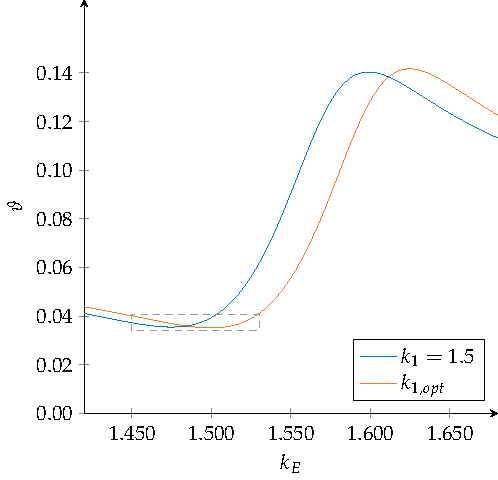
\includegraphics[page=1,width=0.45\textwidth]{TikzNurkoptGanzBereich}}
	\hfill
	\subcaptionbox{Vergrößerte Darstellung des in \figref{fig:Opt:Beispiel:Optimalesk1GanzerBereich} grau gestrichelt gekennzeichneten Bereichs. Durch die Wahl von $k_{1,opt}$ statt $k_1=1.5$ ergibt sich eine Performanceverbesserung von $\D \vartheta = 12.1\%$ an der Stelle $k_E=1.5$
	\label{fig:Opt:Beispiel:Optimalesk1GanzerZoom}}% 
	[0.48\linewidth]{\includegraphics[page=2,width=0.45\textwidth]{TikzNurkoptGanzBereich}}
	
	\caption[Verlauf der Drehungleichförmigkeit als Funktion der Anregungsordnung]{Verlauf der Drehungleichförmigkeit $\vartheta$ für $k_1=1.5$ und $k_{1,opt} = 1.525$ als Funktion der Anregungsordnung $k_E$ mit $\Gamma = \nicefrac{1}{10}$,  $\epsilon = \nicefrac{1}{10}$,  $\delta_1 = 1$}
	\label{fig:Opt:Beispiel:Optimalesk1UeberkE}
\end{figure}
%
%
%
Im hier betrachteten Beispiel soll für ein Standardpendel ohne Mistuning ($u_{1,2}=0$) $\vartheta$ bei $k_E=1.5$ minimal werden. 
Mit den Startwerten $k_{1,0}=1.5$, $I_{a1,0}=2.9 \cdot 10^{-3}$ und $\theta_{a1,0}= 1.3$ für 
$\Gamma = \nicefrac{1}{10}$,  $\epsilon = \nicefrac{1}{10}$ und  $\delta_1 = 1$ ergibt sich das optimale Tuning zu $k_{1,opt} = 1.525$. In \figref{fig:Opt:Beispiel:Optimalesk1UeberkE}  ist
der resultierende Verlauf der Drehungleichförmigkeit $\vartheta$ über der Anregungsordnung $k_E$ für $k_{1,opt} = 1.525$ im
Vergleich zum Verlauf für $k_1 =1.5$  dargestellt. 
Es lässt sich deutlich erkennen, dass das Minimum für den Verlauf mit $k_{1,opt} = 1.525$ 
 bei $k_E = 1.5$ liegt. 
%
Die Wahl von $k_{1,opt}=1.525$ statt $k_1=1.5$ führt dazu, dass sich das Minimum des Verlaufs von $\vartheta$ um
$\D k_E=0.025$ von der Anregungsordnung $k_{E,shift} = 1.475$ zur gewünschten Anregungsordnung $k_E=1.5$ verschiebt.
Mit den hier gewählten Parametern ergibt sich dadurch eine Performanceverbesserung 
von $\D \vartheta = 12.1\%$.
%
Ein mit $k_{1,opt}$ getunter Absorber zeigt  im Gegensatz zu einem mit $k_1 = k_E$ getunten Absorber 
bei der Anregungsordnung $k_E$ eine deutlich bessere Schwingungsreduktionswirkung. 
Allgemein lässt sich auf Basis der hergeleiteten Minimumsbedingung 
immer das optimale Tuning $k_1$ für eine bestimmte Anregungsordnung $k_E$ berechnen,
um dann genau bei dieser Anregungsordnung bestmögliche Performance des Absorbers zu erzielen. 	

%
%
%
%
%
\begin{figure}[ht]%
	\centering
	\subcaptionbox{Verlauf der Drehungleichförmigkeit $\vartheta$ für $k_1=1.5$ und $k_{1,opt} = 1.525$ 
		als Funktion der Anregungsamplitude $\Gamma$ \label{fig:Opt:Beispiel:Optimalesk1UeberGammaDrehunGl}}
	[0.48\textwidth]{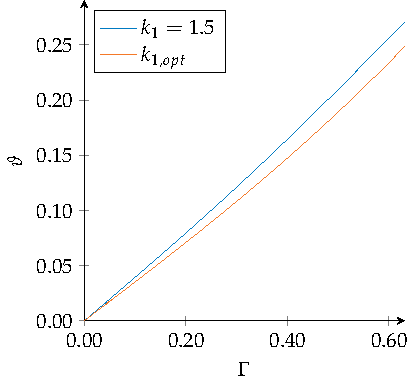
\includegraphics{TikzNurkopt}}
	\hfill
	\subcaptionbox{Prozentuale Performanceverbesserung $\D \vartheta$ des mit $k_{1,opt} = 1.525$  getunten Absorbers gegenüber dem mit $k_1=1.5$ getunten Absorbers \label{fig:Opt:Beispiel:Optimalesk1UeberGammaInProzent}}
	[0.48\textwidth]{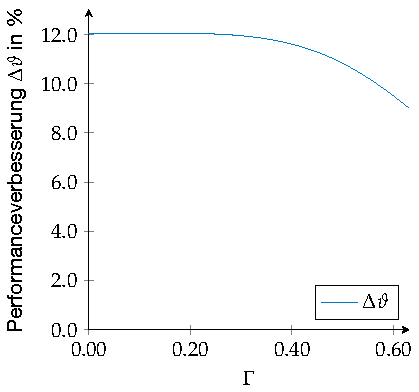
\includegraphics{Vergleichk1Undk1optUeberGammaInProzent-7-7}}
	
	\caption[Verlauf der Drehungleichförmigkeit als Funktion der Anregungsamplitude]{Verlauf der Drehungleichförmigkeit $\vartheta$ für $k_1=1.5$ und $k_{1,opt} = 1.525$ 
				als Funktion der Anregungsamplitude $\Gamma$ mit $k_E = 1.5$,  $\epsilon = \nicefrac{1}{10}$,  $\delta_1 = 1$
				und prozentuale Verbesserung der Performance $\D \vartheta$}
	\label{fig:Opt:Beispiel:Optimalesk1UeberGamma}
\end{figure}
%
%
%
%
%
%
%
\figref{fig:Opt:Beispiel:Optimalesk1UeberGammaDrehunGl} zeigt darüber hinaus, dass die Drehungleichförmigkeit $\vartheta$ für $k_{1,opt} = 1.525$ bei Anregungsordnung $k_E=1.5$ auch
für veränderliche Anregungsamplituden  $\Gamma$  immer kleinere Werte als ein mit $k_1$ getunter Absorber annimmt. 
Der Absorber mit optimalem Tuning $k_{1,opt}$ zeigt bei allen Anregungsamplituden 
bessere Performance als ein mit $k_1=k_E$ getunter Absorber.
In \figref{fig:Opt:Beispiel:Optimalesk1UeberGammaInProzent} ist zur Veranschaulichung
die prozentuale Performanceverbesserung $\D \vartheta$ in Abhängigkeit der
Anregungsamplitude  $\Gamma$ für die verwendeten Parameter dargestellt.


Die beschriebene Optimierung beschränkt sich nicht rein auf die Wahl eines optimalen Tunings $k_1$. 
Ebenso könnten die Parameter im nichtlinearen Mistuning $u_1(s_1)$, wie in den Gleichungen in  \secref{Opt:Bsp:AveragingGleichungen} berücksichtigt, optimiert werden.
Wird beispielsweise $u_1$ als Polynom angesetzt, stellen die Koeffizienten dieses Polynoms weitere Optimierungsparameter dar. 
Beispielsweise tritt für einen Mistuning-Ansatz nach Gleichung 	\eqref{eq:Opt:Bsp:MistAnsatz2terOrdn} in den im 
Optimierungsproblem als Gleichungsnebenbedingungen berücksichtigten Averaging-Gleichungen 	\eqref{eq:OptBspGleichungThetaa1} und \eqref{eq:OptBspGleichungIa1} ein Zusatzterm
durch den Koeffizient $u_{1,2}$ auf und die Zielfunktion $\vartheta$ ist als $\vartheta = \vartheta(k_1,I_{a1},\theta_{a1}, u_{1,2}) $ anzusetzen.
Dies ist bei der Implementierung bereits berücksichtigt.
Eine Erweiterung durch weitere Terme in $u_1(s_1)$ erfolgt analog.
Anderenfalls könnte aber auch von vornherein ein beliebiger Zusammenhang für $u_1(s_1)$ gegeben sein,   
womit wie im dargestellten Beispiel nur $k_{1,opt}$ zu bestimmen ist.  
Dann werden ebenfalls die Averaging-Gleichungen durch die aus dem Mistuning 
resultierenden Terme erweitert, aber die Zielfunktion $\vartheta = \vartheta(k_1,I_{a1},\theta_{a1})$ 
bleibt davon unbeeinflusst.




Zusammenfassend lässt sich festhalten, dass durch die hergeleitete Minimumsbedingung eine Bestimmung des optimalen Tunings $k_1$ möglich ist, jedoch
auch weitere Parameter in den Optimierungsprozess ohne großen Aufwand mit aufgenommen werden können. 









%\newpage
%
%
% SUBOPTIMALES TUNING
%
\subsubsection{Suboptimales Tuning \texorpdfstring{$k_{1,subopt}$}{k1subopt} }

Zu Beginn dieses Abschnitts wurde darauf hingewiesen, dass die Startwerte für $k_1$, $I_{a1}$ und $\theta_{a1}$ im betrachteten Beispiel in der Nähe der erwarteten Lösung zu wählen sind. 
Außerdem wurde gegen Ende von \secref{Opt:Theorie:BestDerGrad} angemerkt, dass es sich bei der Minimumsbedingung \eqref{eq:OptMinimumsbedinungEndg} 
um eine notwendige Bedingung handelt und im Fall, dass Gleichung	\eqref{eq:OptMinimumsbedinungEndg} erfüllt ist bzw.  mehrere Lösungen besitzt, 
die potentiellen Lösungen noch darauf zu prüfen sind, ob ein Minimum vorliegt.
Dies soll zu Abschluss dieses Kapitels genauer betrachtet werden.

Wird die Optimierung mit den (konstruierten) Startwerten $k_{1,0}=1.1$, $I_{a1,0}=7.3 \cdot 10^{-3}$ und $\theta_{a1,0}= 0.05$ bei sonst identischen Parametern  initialisiert, berechnet sich 
das zunächst als optimal erwartete Tuning zu $k_{1,subopt} = 1.405$. 	
%
%
\begin{figure}[bt]%
	\centering
	\begin{subfigure}{0.49\textwidth}
	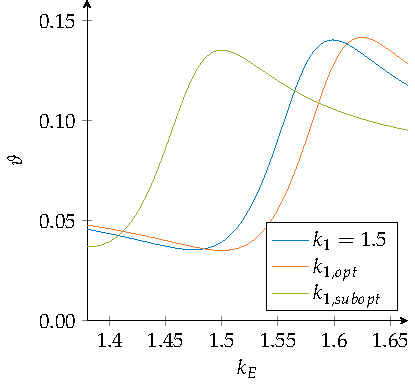
\includegraphics{TikzAuchksubopt-kE} \label{fig:Opt:Beispiel:VerlaufVonVarthetaFuerSuboptimalesk1UeberkE}
	\caption{Verlauf von $\vartheta$ als Funktion der Anregungsordnung $k_E$ für $\Gamma = \nicefrac{1}{10}$}
	\end{subfigure}
	\hfill
	\begin{subfigure}{0.49\textwidth}
	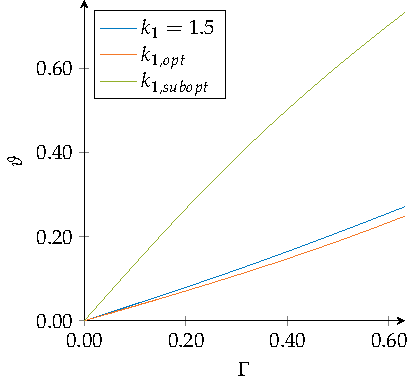
\includegraphics{TikzAuchksubopt-Gamma} \label{fig:Opt:Beispiel:VerlaufVonVarthetaFuerSuboptimalesk1UeberGamma}
	\caption{Verlauf von $\vartheta$ als Funktion der Anregungsamplitude $\Gamma$ für $k_E = 1.5$}
	\end{subfigure}

	\caption[Verlauf der Drehungleichförmigkeit $\vartheta$ für $k_1=1.5$, $k_{1,opt} = 1.525$]
					{Verlauf der Drehungleichförmigkeit $\vartheta$ für $k_1=1.5$, $k_{1,opt} = 1.525$ und $k_{1,subopt}=1.405$ 
					mit $\epsilon = \nicefrac{1}{10}$,  $\delta_1 = 1$;
					$k_{1,opt}$ ist so gewählt, dass das Minimum des Verlaufs von $\vartheta$ bei $k_E=1.5$ liegt; 
					$k_{1,subopt}$ hingegen ist so gewählt, dass das Maximums des Verlaufs von $\vartheta$ bei $k_E=1.5$ liegt	}
	\label{fig:Opt:Beispiel:VerlaufVonVarthetaFuerSuboptimalesk1}
\end{figure}
%
%
%
\figref{fig:Opt:Beispiel:VerlaufVonVarthetaFuerSuboptimalesk1} zeigt die aus 	\figref{fig:Opt:Beispiel:Optimalesk1UeberkE} 
und	\figref{fig:Opt:Beispiel:Optimalesk1UeberGamma} bekannten Graphen mit den für $k_{1,subopt}=1.405$  erweiterten
Verläufen für die Drehungleichförmigkeit $\vartheta$. 
Ein Tuning von $k_{1,subopt}=1.405$ führt im betrachteten Fall dazu, dass sich das Maximum  (und nicht das Minimum)
von $\vartheta$ an der Stelle $k_E=1.5$ befindet (siehe \figref{fig:Opt:Beispiel:VerlaufVonVarthetaFuerSuboptimalesk1UeberkE}), 
was der schlecht möglichsten Absorberperformance an dieser Stelle gleich kommt. Eine extreme Verschlechterung resultiert auch bei
veränderlicher Anregungsamplitude  $\Gamma$ %an allen Stellen 
(vgl. \figref{fig:Opt:Beispiel:VerlaufVonVarthetaFuerSuboptimalesk1UeberGamma}).

Dieses Beispiel verdeutlicht, dass durch die notwendige Bedingung \eqref{eq:OptMinimumsbedinungEndg} bei Initialisierung mit
ungünstigen Anfangswerten auch eine
Lösung für das Tuning berechnet werden kann, welche ein Maximum  von $\vartheta$ an einer bestimmten Stelle $k_E$ zur Folge hat.
Um dies zu vermeiden, ist es von großer Bedeutung die Optimierung mit sinnvollen Anfangswerten zu initialisieren (vgl. Anmerkungen zu Beginn dieses
Abschnitts) und im Anschluss daran zu prüfen, ob wirklich das optimale Tuning berechnet wurde.


\chapter{Zusammenfassung und Ausblick}
\label{cha:Schluss}

Im Rahmen der vorliegenden Masterarbeit wurden 
Untersuchungen zur optimalen Auslegung von Fliehkraftpendeln durchgeführt.


Es wurde allgemein hergeleitet, wie das optimale lineare Tuning $k$
eines Fliehkraftpendels zu bestimmen ist, was nun direkt in den Entwurfsprozess
aufgenommen werden kann.
Untersuchungen des Einflusses eines verallgemeinerten Rotationsgradienten 
und  des Einflusses von  nichtlinearem Mistuning auf das Systemverhalten wurden durchgeführt.
Aus den dabei gewonnenen Erkenntnissen wurden
Aussagen und Vorschläge zur gezielten Beeinflussung und Optimierung
der Fliehkraftpendelwirkung durch spezielle Wahl des Rotationsgradienten
und des Mistunings abgeleitet.




% Zusammenfassung der Punkte
%%%%%%%%%%%%%%%%%%%%%%%%%%%%%%%%%%%%%%%%%%%
% Simulation und Bogenlängenverfahren
Die Untersuchungen wurden auf Basis der Averaging-Gleichungen, welche eine 
Approximation der stationären Systemantwort  darstellen,  durchgeführt.
Da die Systemantwort stark nichtlineares Verhalten mit kritischen Punkten
(horizontale und vertikale Tangenten im Gleichgewichtspfad) aufweist, ist
es nicht möglich diese in geschlossener Form zu lösen.
Um eine systematische, numerische Lösung der Gleichungen zu ermöglichen und etwaige 
Schwierigkeiten klassischer Lösungsverfahren bei kritischen Punkten
zu vermeiden, wurde in dieser Arbeit ein Bogenlängenverfahren implementiert,
welches bei den weiteren Untersuchungen zur Anwendung kam.
Darüber hinaus wurde ein Simulationsprogramm erstellt, 
mit welchem  die Aussagekraft der auf Basis der Averaging-Gleichungen 
prognostizierten  Systemantwort durch Vergleich mit den Ergebnissen 
aus der Simulation der vollständigen, nichtlinearen 
Bewegungsgleichungen des dynamischen Fliehkraftpendelsystems
verifiziert wurde.




% Optimales Tuning
Die Schwingungsreduktionswirkung eines Fliehkraftpendels mit linearem Tuning $k=k_E$ 
ist durch den Einfluss von viskoser Dämpfung  bei der Anregungsordnung $k_E$ nicht optimal.
Das gedämpfte Fliehkraftpendel zeigt nicht bei der Anregungsordnung $k_E$ beste Wirkung,
sondern der Punkt bester Absorberwirkung verschiebt sich zu einer 
anderen Anregungsordnung. 
Durch die Wahl des Absorbertunings $k$ wird eine Veränderung der Geometrie und somit
eine Veränderung der Dynamik erreicht, womit
dem ungewünschten Einfluss der viskosen Dämpfung entgegengewirkt werden kann. 
In dieser Arbeit wurde eine  analytische Bedingung, mit welcher das optimale Tuning $k$ eines
Fliehkraftpendels unter Berücksichtigung linear viskoser Dämpfung bestimmt
und somit direkt im Entwurfsprozess berücksichtigt werden kann, hergeleitet.
%
Damit kann nun  bereits im Auslegungsprozess dem suboptimalen Einfluss der Dämpfung 
vorgebeugt und optimale Absorberwirkung bei der auftretenden 
Anregungsordnung $k_E$ erreicht werden.  
%
Durch den aus der analytischen Bedingung berechneten Wert für das optimale 
Tuning $k$ bleibt die tautochrone Eigenschaft des Fliehkraftpendels erhalten
und es besitzt optimale Schwingungsreduktionswirkung bei der
auftretenden Anregungsordnung. 

 
% Rotationsgradient
In dieser Arbeit wurde der in \cite{Mayet:Tautochronic} als 
konstant vorgeschlagene Gradient $\frac{\partial \bar{\alpha}}{\partial s}$ 
als Reihe angesetzt und damit der Einfluss eines verallgemeinerten Rotationsgradienten 
auf die Absorberwirkung untersucht. 
Auf Basis der Averaging-Gleichungen konnte für die im Rahmen dieser Arbeit getroffenen
Ansätze durch den verallgemeinerten Rotationsgradienten eine scheinbare
Verbesserung der Absorberperformance erzielt werden, welche allerdings durch die
vollständige Simulation nicht bestätigt werden konnte.
Die Averaging-Gleichungen bildeten unter Berücksichtigung des verallgemeinerten Rotationsgradienten das Systemverhalten 
nur in äußerst kleinen Bereichen hinreichend  genau ab.
Auch bei der Erweiterung der getroffenen Ansätze um Terme höherer Ordnung
konnte keine Verbesserung der Absorberperformance %durch einen verallgemeinerten Rotationsgradienten 
erreicht werden. 
Die in dieser Arbeit durchgeführten Untersuchungen bestätigten, dass für ein Rotationspendel
mit den im Rahmen dieser Arbeit zugrunde gelegten  Ansätzen die Wahl von  
$\frac{\partial \bar{\alpha}}{\partial s} = \sqrt{\mu_r/(1+\mu_r)}= \const$,
wie in \cite{Mayet:Tautochronic} vorgeschlagen, wahrscheinlich
optimal ist. 
Diese Erkenntnis wurde bei der weiteren Untersuchung des Einflusses von
nichtlinearem Mistuning berücksichtigt. 

% Untersuchung Mistuning
Durch den gezielten Einsatz von nichtlinearem Mistuning konnte die Robustheit
eines Absorbers  gegenüber Änderungen in der Anregungsordnung deutlich gesteigert werden.
Dabei wird der Anstieg der Absorberamplitude und der  Drehungleichförmigkeit 
zu deutlich größeren Anregungsordnungen verschoben.
Dadurch wurde die Gefahr zum Sprung in der Absorberamplitude, welche für
ein Kreisbahnpendel typisch ist und wozu ein tautochrones Rotationspendel 
auch tendiert, deutlich abgemildert. 
Die drastische Performanceverschlechterung, welche beim Sprung
der Absorberamplitude zwangsweise auftreten würde, wurde damit unterbunden.
Des Weiteren wird beim Einsatz von nichtlinearem Mistuning die Performance 
bei der Anregungsordnung, für welche das Fliehkraftpendel ausgelegt ist,
im Rahmen der Näherung durch die Averaging-Gleichungen nicht beeinflusst.
Der Einfluss des auf Basis der Averaging-Gleichungen ermittelten Vorschlags für das
nichtlineare Mis"-tuning konnte durch die nichtlineare, vollständige Simulation bestätigt werden. 
Da das prognostizierte Systemverhalten durch die Averaging-Gleichungen 
nahezu identisch mit  den Ergebnissen der Simulation ist,
wird das stationäre Absorberverhalten durch die Averaging-Gleichungen sehr gut approximiert.
Die auf Basis der Averaging-Gleichungen unter Berücksichtigung von 
nichtlinearem Mistuning prognostizierte Absorberantwort ist als Auslegungskriterium für den Fliehkraftpendelentwurf
sehr gut geeignet.


Im Rahmen dieser Arbeit konnte das Verhalten mehrerer Fliehkraftpendel
und die damit verbundenen Effekte wie beispielsweise asynchrones Verhalten
nicht untersucht werden. 
Eine mögliche und vielversprechende Anwendung wäre der Einsatz von 
nichtlinearem Mis"-tuning bei Absorbersystemen mit mehreren Freiheitsgraden.
Dabei könnte das nichtlineare Mistuning signifikante Effekte bezüglich
der Vermeidung von asynchronen Pendelbewegungen besitzen.
Zur genauen  Beurteilung solcher Effekte sind aber noch detaillierte Untersuchungen nötig.




\backmatter
\chapter{Averaging-Methode} \label{ap:Averaging}



Die \new{Averaging-Methode} oder  \new{Methode der Mittelwertbildung} (engl. \textit{averaging method}) wird zur Analyse 
nichtlinearer Oszillationen eines dynamischen Systems verwendet \cite{Mitropolsky:Averaging}. 
Die Grundidee der Methode ist die Approximation des Ausgangssystems durch ein gemitteltes System, welches dadurch 
deutlich einfacher zu untersuchen ist \cite{Hagedorn:NichtlinSchwingungen1978}.
Aus dem Verständnis der Dynamik des gemittelten Systems  können Rückschlüsse auf die 
Dynamik des Ausgangssystems gezogen werden  \cite{Hagedorn:NichtlinSchwingungen1978}. 
Dabei wird durch Zeitintegration über eine Periode des Ausgangssystems  der Einfluss der hochfrequenten Dynamiken 
herausgefiltert \cite{Hagedorn:NichtlinSchwingungen1978}. 
Die wichtigsten Zusammenhänge zur praktischen Anwendung, wie sie im Rahmen der Herleitungen in dieser Arbeit 
benötigt werden, sind im Folgenden kurz dargelegt, wobei hier die einfachste Form der Mittelwertbildung, 
die \textit{periodische Mittelwertbildung} \cite{Sanders:AveragingMethods2007}, betrachtet wird. 
Die  angegebenen Zusammenhänge geben den Grundgedanken der Averaging-Methode wieder.
Weitere Details, Beweise und Verallgemeinerungen sind in \cite{Sanders:AveragingMethods2007} zu finden. 

Ausgegangen wird von einem System in der Form
\begin{equation}
	\vec{\dot{x}} = \epsilon \vf\left(\vx,t\right) + \mathcal{O}(\epsilon^2), \qquad  \vx\left(0\right) = \va,
\label{eq:AveragingAusgangsgleichung}
\end{equation}
wobei $\epsilon$ ein kleiner Parameter und $\vf$ ein $T$-periodisches Vektorfeld in der Zeit $t$ ist.

Vernachlässigung von Termen höherer Ordnung und Mittelwertbildung durch Integration über $t$ führt auf die \textit{gemittelte Gleichung}
\begin{equation}
	\vec{\dot{z}} = \epsilon \vec{\bar{f}}\left(\vz\right), \qquad  \vz\left(0\right) = \va, 
\label{eq:AveragingGemittelteGleichung}
\end{equation}
%
%
mit
%
%
\begin{equation}
	\vec{\bar{f}}\left(\vz\right) = \frac{1}{T} \int^T_0{\vf\left(\vz,s\right) \dd s} .
\label{eq:AveragingGemittelteGleichungRechteSeite}
\end{equation}
%
%
%
Das grundlegende Ergebnis dieser Mittelung ist, dass die Lösungen des gemittelten Systems nahe (von Ordnung $\epsilon$) 
an den Lösungen des Ausgangssystems in einem Zeitintervall der Ordnung $1/\epsilon$ sind \cite{Sanders:AveragingMethods2007}, was sich als
\begin{equation}
	\left\| \vx\left(t\right) - \vz\left(t\right) \right\| \leq c \epsilon \quad \text{für} \quad 0 \leq t \leq \frac{L}{\epsilon}
\label{eq:AveragingEpsilonNah}
\end{equation}
mit positiven Konstanten $c$ und $L$ schreiben lässt. Unter weiter spezifizierten Anforderungen, 
welche für reale Systeme in der Regel zutreffen, bleiben die Lösungen des gemittelten Systems 
auch für das Zeitintervall $t \in \left[0, \infty \right)$ nahe (von Ordnung $\epsilon$) 
an den Lösungen des Ausgangssystems \cite{Sanders:AveragingMethods2007}.







\chapter{Rotationspendel} \label{ap:Rotationspendel}



Im Folgenden wird das Beispiel zum rotierenden Pendel aus \cite{Mayet:Tautochronic} dargelegt, 
da die dort hergeleiteten Sachverhalte 
als wichtige Grundlage für die im Rahmen dieser Arbeit durchgeführten Untersuchungen dienen.
Betrachtet wird ein einzelnes Pendel ($n_p = 1$), welches die Möglichkeit hat, im rotorfesten
Koordinatensystem zu rotieren ($\mu_r \neq 0$). 
%
Die geometrische Zwangsbedingung für ein solches Pendel ergibt sich nach \secref{subsec:TautDesignBedingungen} zu
\begin{equation}
		\left(\pdiff{\rho}{s}\right)^2 +  \rho^2 \left(\pdiff{\varphi}{s}\right)^2    + \mu_{r} \left(\pdiff{\alpha}{s}\right)^2  = 1.
				\label{eq:AnhTautochronerAbsorberentwurfGeomZwangsbedRotPendel}
\end{equation}




Werden die Lösungen $\varphi$, für welche kein Rotationsgradient $\pdiff{\alpha}{s}$ auftritt, mit $\varphi_0$ bezeichnet, 
resultiert die Zwangsbedingung für diesen Fall zu
\begin{equation}
		\left(\pdiff{\rho}{s}\right)^2 +  \rho^2 \left(\pdiff{\varphi_0}{s}\right)^2  = 1
				\label{eq:AnhTautochronerAbsorberentwurfGeomZwangsbedRotPendelOhneRot}
\end{equation}
und für $\varphi_0$ gilt mit dem skalierten Radius $\rho^2(s) = 1 - k^2 s^2$ explizit
\begin{equation}
		\left(\pdiff{\varphi_0}{s}\right)^2  = \frac{1}{\rho^2}  \left(   1 - \left(\pdiff{\rho}{s}\right)^2    \right),
				\label{eq:AnhTautochronerAbsorberentwurfGeomZwangsbedDefPhi0}
\end{equation}
wofür eine analytische Lösung existiert, welche in \cite{Mayet:Tautochronic} angegeben ist.
%
%
%
% Geom. Zwangsbedingung für Rotationspendel
%
Mit dieser Definition lautet die geometrische Zwangsbedingung für $\varphi$ für ein rotierendes Pendel
\begin{equation}
		\left(\pdiff{\varphi}{s}\right)^2  =  \left(\pdiff{\varphi_0}{s}\right)^2     -   \frac{\mu_r}{\rho^2} \left(\pdiff{\alpha}{s}\right)^2.   
				\label{eq:AnhTautochronerAbsorberentwurfGeomZwangsbedDefPhi}
\end{equation}
%
%
% Ansatz für Rotationsgradien
%
Der Rotationsgradient wird in \cite{Mayet:Tautochronic} als
\begin{equation}
		\pdiff{\alpha}{s}  = \frac{\rho}{\sqrt{\mu_r}}   \pdiff{\varphi_0}{s} \pdiff{\bar{\alpha}}{s}   
		\qquad \text{mit} \qquad 			  \left| \pdiff{\bar{\alpha}}{s} \right|  < 1 \quad \forall s
				\label{eq:AnhTautochronerAbsorberentwurfAnsatzRotationsgradient}
\end{equation}
%
angesetzt, wobei $\bar{\alpha}(s)$ eine beliebige Funktion von $s$ und deren Betrag kleiner als 1 ist. Damit resultiert
\begin{equation}
		\pdiff{\varphi}{s} =  \pdiff{\varphi_0}{s}  \sqrt{  1 - \left(\pdiff{\bar{\alpha}}{s}\right)^2  },
				\label{eq:AnhTautochronerAbsorberentwurfGeomZwangsbedDefPhiMitSpezAlpha}
\end{equation}
%
wobei jedoch für $\varphi$ keine allgemeine Lösung mehr existiert. Diese wird auch nicht zwingend benötigt, da für das dynamische Verhalten des Systems nur der Rotationsgradient entscheidend ist, wie anhand der Definition von $f(s)$ ersichtlich ist. 
$f(s)$ ergibt sich nach Gleichung 	\eqref{eq:Abkuerzungenfuerf} unter Verwendung der eben dargestellten Definitionen   für ein Rotationspendel zu
%
%
% Defintion von f(s)
%
\begin{equation}
	\begin{split}
		f(s) &= \rho^2 \pdiff{\varphi}{s} + \mu_r \pdiff{\alpha}{s}
				  = \rho^2 \pdiff{\varphi_0}{s}  \sqrt{  1 - \left(\pdiff{\bar{\alpha}}{s}\right)^2  } + \mu_r \frac{\rho}{\sqrt{\mu_r}}   \pdiff{\varphi_0}{s} \pdiff{\bar{\alpha}}{s}  \\
				 &= \pdiff{\varphi_0}{s} \left(\rho^2 \sqrt{  1 - \left(\pdiff{\bar{\alpha}}{s}\right)^2} + \sqrt{\mu_r} \rho  \pdiff{\bar{\alpha}}{s}  \right)	.
				\label{eq:AnhTautochronerAbsorberentwurfDefVonf}
	\end{split}				
\end{equation}
%
In \cite{Mayet:Tautochronic}  wird vorgeschlagen, den Gradienten von $\bar{\alpha}$ %der Einfachheit halber
konstant zu wählen. 
Die Wahl von 
\begin{equation}
		 \pdiff{\bar{\alpha}}{s} = \sqrt{\frac{\mu_r}{1+\mu_r}}
				\label{eq:AnhTautochronerAbsorberentwurfWahlVonAlphaS}
\end{equation}
maximiert die Funktion $f(s)$ an der Stelle $s=0$, was die Wirkung des Absorbers bei kleinen Amplituden erhöht \cite{Mayet:Tautochronic}.
Für die Wahl von  $\pdiff{\bar{\alpha}}{s} = \const$ ergeben sich die Lösungen von $\varphi$ durch Multiplikation von $\varphi_0$
mit einer Konstanten und die resultierende Funktion $f(s)$ lautet 
%
%
% Resultierendes f(s)
%
\begin{equation}
		 f(s) = \sqrt{1+\mu_r} - \frac{k^2}{2 \sqrt{\mu_r+1}} \left(\left(\mu_r + 1\right) k^2 + 1 \right) s^2 +  \mathcal{O}(s^4),
			\label{eq:AnhTautochronerAbsorberentwurfFendgueltig}
\end{equation}
welche für weitere Untersuchungen allgemein als 
\begin{equation}
		 f(s) = b_0 + b_2 s^2 +  \mathcal{O}(s^4) \qquad \text{mit} \qquad b_0, b_2 \in \MR
			\label{eq:AnhTautochronerAbsorberentwurfFAlsPolynom}
\end{equation}
geschrieben wird.



\AMPrintBibliography
\end{document}

% Compilation process:
pdflatex Masterarbeit.tex
biber Masterarbeit
pdflatex Masterarbeit.tex
pdflatex Masterarbeit.tex
